%!TEX root = ../nwoods_thesis.tex

\chapter{ZZ Phenomenology and Previous Results}\label{ch:pheno}

Four-lepton final states originate primarily from three physics processes: nonresonant diboson production, resonant Higgs boson production which decays to {\ZZs}, and resonant single-{\PZ} production.
Multi-{\PZ} triboson production ({\WZZ} and {\ZZZ}) occurs at negligible rates~\cite{Lazopoulos:2007ix,Binoth:2008kt}.
Single-{\PZ} triboson production ({\WWZ})~\cite{Hankele:2007sb,Binoth:2008kt} and {\TTZ} production result in final states with four prompt leptons, but are considered background (see Section~\ref{sec:bkgPheno}).
The three signal processes can be distinguished by kinematics, such as the four-lepton invariant mass distribution.

The signal processes all involve on- or off-shell {\PZ} bosons.
The {\PZ} was first indirectly observed in 1973 when the Gargamelle bubble chamber experiment at CERN recorded an elastic muon antineutrino-electron ($\Panm + \Pe^- \to \Panm + \Pe^-$) scattering event~\cite{Hasert:1973cr}.
Direct observation in leptonic decays came roughly a decade later, from the UA1 experiment, also at CERN~\cite{Arnison:1983mk}.
Clean {\epem} collisions at LEP and SLAC, where the center-of-mass energy could be adjusted to produce {\PZ} bosons copiously, allowed its properties---and a number of other parameters of the electroweak theory---to be measured with per-mille precision or better~\cite{ALEPH:2005ab}.
Of particular importance to this study, the {\PZ} mass is
\begin{equation}
  m_\PZ = 91.1876 \pm 0.0021\GeV,
\end{equation}
its full width is
\begin{equation}
  \Gamma_\PZ = 2.4952 \pm 0.0023\GeV,
\end{equation}
its width in leptonic decays is
\begin{equation}
  \Gamma_\PZ (\ell^+\ell^-) = 83.984 \pm 0.086\MeV,
\end{equation}
and it decays to a pair of charged leptons 3.3658\% of the time for each lepton flavor~\cite{Olive:2016xmw}.



\section[Nonresonant
         \texorpdfstring{$\mathrm{ZZ/Z}\gamma^\ast$}{ZZ/Zgamma*}
         Production and Decay]{Nonresonant $\mathbf{ZZ/Z}\gamma^\ast$ Production and Decay}

Leading-order {\ZZ} production is {\qqb}-initiated and proceeds through $t$-channel quark exchange, as shown in Fig.~\ref{fig:zzLO}.
At next-to-leading order (NLO\@; several representative diagrams are shown in Fig.~\ref{fig:zzNLO}), production may have a gluon in the initial state and may have a quark or gluon in the final state which hadronizes and appears experimentally as a jet~\cite{Campbell:1999ah,Campbell:2011bn,Melia:2011tj}.
Next-to-next-to-leading order (NNLO) adds gluon-gluon fusion box diagrams (Fig.~\ref{fig:zzBox}), as well as {\qqb}-initiated production with two loops, one loop and a final state jet, and two jets~\cite{Cascioli:2014yka,Caola:2015psa}.
The NLO and NNLO corrections are generally large, outside the scale uncertainties of the calculations at previous orders, because diagrams with new initial states contribute only positively to the cross section.
Quark-gluon scattering diagrams introduced at NLO and gluon-gluon fusion diagrams introduced at NNLO have large amplitudes---the $\Pgg \to \ZZ$ process accounts for roughly 60\% of the total NNLO correction, for example---due to the high effective gluon luminosity in multi-{\TeVns} proton collisions~\cite{Cascioli:2014yka}.
Because of the box diagrams' large contribution, ``$\text{NLO} + \Pgg$'' simulations are often used, in which NLO $\qqb/\Pq\Pg/\Paq\Pg \to \ZZ$ and LO $\Pgg \to \ZZ$ samples are summed even though they formally contribute at different orders in {\alphaS}.

\begin{figure}[htbp]
  \vspace{1em}
  \begin{center}
    \begin{fmffile}{zzLO}
      \begin{fmfgraph*}(0.26,0.26) % chktex 36
        \fmfstraight %chktex 1
        \fmfleft{i1,d1,d2,i2}
        \fmfright{o1,o2,o3,o4}
        \fmflabel{\Pq}{i1}
        \fmflabel{\Paq}{i2}
        \fmflabel{\Plpp}{o1}
        \fmflabel{\Plpm}{o2}
        \fmflabel{\Plp}{o3}
        \fmflabel{\Plm}{o4}
        \fmf{fermion}{i1,v1,v2,i2}
        \fmf{zigzag,label={\PZ}}{v1,v3}
        \fmf{zigzag,label={\PZ},label.side=left}{v2,v4}
        \fmf{fermion}{o1,v3,o2}
        \fmf{fermion}{o3,v4,o4}
      \end{fmfgraph*}
    \end{fmffile}
    \hspace{4em}
      \begin{fmffile}{zzOL}
        \begin{fmfgraph*}(0.26,0.26) % chktex 36
          \fmfstraight %chktex 1
          \fmfleft{i1,d1,d2,i2}
          \fmfright{o1,o2,o3,o4}
          \fmflabel{\Pq}{i1}
          \fmflabel{\Paq}{i2}
          \fmflabel{\Plpp}{o1}
          \fmflabel{\Plpm}{o2}
          \fmflabel{\Plp}{o3}
          \fmflabel{\Plm}{o4}
          \fmf{fermion}{i1,v1,v2,i2}
          \fmf{phantom}{v1,v3}
          \fmf{phantom}{v2,v4}
          \fmf{fermion}{o1,v3,o2}
          \fmf{fermion}{o3,v4,o4}
          \fmffreeze % chktex 1
          \fmf{zigzag}{v1,v4}
          \fmf{zigzag}{v2,v3}
          \fmf{phantom}{v1,v6}
          \fmf{phantom}{v2,v5}
          \fmf{phantom,label={\PZ},tension=2,l.s=left}{v6,v4}
          \fmf{phantom,label={\PZ},tension=2,l.s=right}{v5,v3}
        \end{fmfgraph*}
      \end{fmffile}
    \vspace{1em}
    \caption[Leading order {\ZZfourl} production]{
      Leading order Feynman diagrams for {\ZZfourl} production in {\pp} collisions.
      }\label{fig:zzLO}
  \end{center}
\end{figure}

\begin{figure}[htbp]
  \vspace{1em}
  \begin{center}
    \begin{fmffile}{zzNLOg}
      \begin{fmfgraph*}(0.26,0.26) % chktex 36
        \fmfstraight %chktex 1
        \fmfleft{i1,d1,d2,d3,i2}
        \fmfright{o1,o2,o3,o4,o5}
        \fmflabel{\Pq}{i1}
        \fmflabel{\Paq}{i2}
        \fmflabel{\Plpp}{o1}
        \fmflabel{\Plpm}{o2}
        \fmflabel{\Pg}{o3}
        \fmflabel{\Plp}{o4}
        \fmflabel{\Plm}{o5}
        \fmf{fermion}{i1,v1,v2,v3,i2}
        \fmf{phantom,tension=0.4}{v1,o1}
        \fmf{phantom,tension=0.4}{v2,o3}
        \fmf{phantom,tension=0.4}{v3,o5}
        \fmffreeze % chktex 1
        \fmf{zigzag,label={\PZ}}{v1,v4}
        \fmf{zigzag,label={\PZ},l.s=left}{v3,v5}
        \fmf{gluon}{v2,o3}
        \fmf{fermion}{o1,v4,o2}
        \fmf{fermion}{o4,v5,o5}
      \end{fmfgraph*}
    \end{fmffile}
    \hspace{4em}
    \begin{fmffile}{zzNLOLoop}
      \begin{fmfgraph*}(0.26,0.26) % chktex 36
        \fmfstraight %chktex 1
        \fmfleft{i1,d1,d2,i2}
        \fmfright{o1,o2,o3,o4}
        \fmflabel{\Pq}{i1}
        \fmflabel{\Paq}{i2}
        \fmflabel{\Plpp}{o1}
        \fmflabel{\Plpm}{o2}
        \fmflabel{\Plp}{o3}
        \fmflabel{\Plm}{o4}
        \fmf{fermion}{i1,v1,v2,v3,v4,i2}
        \fmf{gluon}{v1,v4}
        \fmf{phantom}{v2,o1}
        \fmf{phantom}{v3,o4}
        \fmffreeze % chktex 1
        \fmf{zigzag,label={\PZ},l.s=right}{v2,v5}
        \fmf{zigzag,label={\PZ},l.s=left}{v3,v6}
        \fmf{fermion}{o1,v5,o2}
        \fmf{fermion}{o3,v6,o4}
      \end{fmfgraph*}
    \end{fmffile}
    \vspace{4em}

    \begin{fmffile}{zzNLOq}
      \begin{fmfgraph*}(0.26,0.26) % chktex 36
        \fmfstraight %chktex 1
        \fmfleft{i1,d1,d2,d3,d4,i2}
        \fmfright{o1,o2,o3,o4,d5,o5}
        \fmfright{d6,d7,d8}
        \fmflabel{\Pq}{i1}
        \fmflabel{\Pg}{i2}
        \fmflabel{\Plpp}{o1}
        \fmflabel{\Plpm}{o2}
        \fmflabel{\Plp}{o3}
        \fmflabel{\Plm}{o4}
        \fmflabel{\Pq}{o5}
        \fmf{fermion}{i1,v1,v2,v3}
        \fmf{fermion,tension=0.4}{v3,o5}
        \fmf{phantom,tension=0.4}{v1,o1}
        \fmf{phantom,tension=0.4}{v2,d7}
        \fmf{gluon}{i2,v3}
        \fmffreeze % chktex 1
        \fmf{zigzag,label={\PZ}}{v1,v4}
        \fmf{zigzag,label={\PZ}}{v2,v5}
        \fmf{fermion}{o1,v4,o2}
        \fmf{fermion}{o3,v5,o4}
      \end{fmfgraph*}
    \end{fmffile}
    \hspace{4em}
    \begin{fmffile}{zzNLOaq}
      \begin{fmfgraph*}(0.26,0.26) % chktex 36
        \fmfstraight %chktex 1
        \fmfleft{i1,d1,d2,d3,d4,i2}
        \fmfright{o1,o2,o3,o4,d5,o5}
        \fmfright{d6,d7,d8}
        \fmflabel{\Paq}{i1}
        \fmflabel{\Pg}{i2}
        \fmflabel{\Plpp}{o1}
        \fmflabel{\Plpm}{o2}
        \fmflabel{\Plp}{o3}
        \fmflabel{\Plm}{o4}
        \fmflabel{\Paq}{o5}
        \fmf{fermion}{v3,v2,v1,i1}
        \fmf{fermion,tension=0.4}{o5,v3}
        \fmf{phantom,tension=0.4}{o1,v1}
        \fmf{phantom,tension=0.4}{d7,v2}
        \fmf{gluon}{i2,v3}
        \fmffreeze % chktex 1
        \fmf{zigzag,label={\PZ}}{v1,v4}
        \fmf{zigzag,label={\PZ}}{v2,v5}
        \fmf{fermion}{o1,v4,o2}
        \fmf{fermion}{o3,v5,o4}
      \end{fmfgraph*}
    \end{fmffile}
    \vspace{1em}
    \caption[Next-to-leading order {\ZZfourl} production]{
      Four representative Feynman diagrams that contribute to {\ZZfourl} production in {\pp} collisions at NLO\@.
      Clockwise from the top right, the diagrams are examples of one-loop diagrams, real antiquark and quark emission, and real gluon emission.
      The loop diagram (top right) is formally NNLO, but contributes at NLO through interference with NLO $\qqb \to \ZZ$ diagrams.
      }\label{fig:zzNLO}
  \end{center}
\end{figure}

\begin{figure}[htbp]
  \vspace{1em}
  \begin{center}
    \begin{fmffile}{zzBox}
      \begin{fmfgraph*}(0.325,0.25) % chktex 36
        \fmfstraight %chktex 1
        \fmfleft{i1,i2}
        \fmfright{o1,o2,o3,o4}
        \fmflabel{\Pg}{i1}
        \fmflabel{\Pg}{i2}
        \fmflabel{\Plpp}{o1}
        \fmflabel{\Plpm}{o2}
        \fmflabel{\Plp}{o3}
        \fmflabel{\Plm}{o4}
        \fmf{gluon}{i1,v1}
        \fmf{gluon}{i2,v2}
        \fmf{phantom}{v3,o4}
        \fmf{phantom}{v4,o1}
        \fmf{fermion}{v3,v4,v1,v2}
        \fmf{fermion,label={\Pq}}{v2,v3}
        \fmffreeze % chktex 1
        \fmf{zigzag,label={\PZ}}{v3,v6}
        \fmf{zigzag,label={\PZ}}{v4,v5}
        \fmf{fermion}{o1,v5,o2}
        \fmf{fermion}{o3,v6,o4}
      \end{fmfgraph*}
    \end{fmffile}
    \vspace{1em}
    \caption[Gluon-gluon fusion box diagram for {\ZZfourl} production]{
      A LO box diagram for {\ZZfourl} production through a quark loop in a gluon-gluon fusion event.
      This is formally an NNLO diagram for {\ZZ} production overall, but is often included in NLO calculations because it accounts for a large fraction of the NNLO correction and its contribution to the {\ZZ} cross section has a similar magnitude to that from the NLO corrections.
      The {$\Pgg \to \ZZ$} amplitude is so large due to the high effective luminosity of gluons with enough energy to produce a {\PZ} boson pair in proton collisions at high $Q^2$,
      }\label{fig:zzBox}
  \end{center}
\end{figure}

Production of pairs of on-shell {\PZ} bosons\footnote{Events with two on-shell {\PZ} bosons are often called ``doubly resonant,'' but are a subset of ``nonresonant'' production in the sense that the {\ZZ} system is not produced by a resonance. Either term may be used to distinguish ``continuum'' production from ``singly resonant'' production from {\Zfourl}, $\PH \to \ZZ^\ast$, or a potential new particle which decays to {\ZZ}.} turns on sharply at the kinematic threshold $\sqrt{\hat{s}} = 2m_{\PZ} = 182.4\GeV$, and in proton-proton collisions at $\sqrt{s} = 13\TeV$, peaks around $m_{\ZZ} \approx 200\GeV$ before falling steeply at higher invariant masses.
Continuum production occurs below the kinematic threshold when one or both {\PZ} bosons are replaced by a $\PZ^\ast / \Pa^\ast$ admixture, typically in the form of a $\qqb \to \PZ$ event in which one of the incoming quarks emits a virtual photon as initial state radiation (ISR).
Events of interest in this analysis (see Sections~\ref{sec:zzSelection} and~\ref{sec:xSecCalc}) generally have one on-shell {\PZ}, and a $\PZ^\ast/\Pa^\ast$ at a lower mass.
Nonresonant $\PZ\Pa^\ast$ production is generally flat as a function of invariant mass between roughly {100\GeV} and the doubly resonant threshold.


\subsection{Vector Boson Scattering}

Vector boson scattering proceeds at hadron colliders through the diagrams shown in Fig~\ref{fig:vbs}, resulting in a {\ZZjj} final state.
This fully electroweak (EWK) production must be distinguished from the background of QCD-initiated $\ZZ + \text{jets}$ events (see Section~\ref{sec:bkgPheno}).
The hallmark of the EWK process is a pair of high energy, high rapidity jets from the quarks, which retain a high boost along the $z$-axis even after electroweak boson emission and are thus deflected through a small angle in the lab frame.
At the same time, the {\ZZ} system is produced with low transverse boost compared to QCD-initiated {\ZZjj} events, in which the {\ZZ} system recoils against the jets, and somewhat higher invariant mass on average~\cite{Zeppenfeld:54.6680}.
Because the hard scattering interaction involves no color exchange or reconnection~\cite{Zeppenfeld:54.6680,Sjostrand:2014zea,Bierlich:2015rha}, VBS events are much less likely to have less energetic jets between the two high-energy quark jets.
Useful variables to discriminate between EWK and QCD production therefore include the angle between the jets, the jet energies, the dijet invariant mass, the {\ZZ} invariant mass and rapidity, and the number of central jets (see Section~\ref{sec:vbsSearch} for a full list and definitions).

\begin{figure}[htbp]
  \vspace{1em}
  \begin{center}
    \begin{fmffile}{vbsTGC}
      \begin{fmfgraph*}(0.3,0.25) % chktex 36
        \fmfstraight %chktex 1
        \fmfleft{i1,d1,d2,i2}
        \fmfright{o1,o2,o3,o4,o5,o6}
        \fmflabel{$\Pq_1$}{i1}
        \fmflabel{$\Pq_2$}{i2}
        \fmflabel{$\Pq_1^\prime$}{o1}
        \fmflabel{$\Pq_2^\prime$}{o6}
        \fmflabel{\Plpp}{o2}
        \fmflabel{\Plpm}{o3}
        \fmflabel{\Plp}{o4}
        \fmflabel{\Plm}{o5}
        \fmf{fermion}{i1,v1,o1}
        \fmf{zigzag}{v1,v2}
        \fmf{zigzag,label={\PWpm},label.side=left}{v2,v3}
        \fmf{zigzag}{v3,v4}
        \fmf{fermion}{i2,v4,o6}
        \fmf{phantom}{d1,v1}
        \fmf{phantom}{d2,v4}
        \fmffreeze % chktex 1
        \fmf{zigzag,label={\PZ}}{v2,v5}
        \fmf{zigzag,label={\PZ}}{v3,v6}
        \fmf{fermion}{o2,v5,o3}
        \fmf{fermion}{o4,v6,o5}
      \end{fmfgraph*}
    \end{fmffile}
    \hspace{4em}
    \begin{fmffile}{vbsQGC}
      \begin{fmfgraph*}(0.3,0.25) % chktex 36
        \fmfstraight %chktex 1
        \fmfleft{i1,d1,d2,i2}
        \fmfright{o1,o2,o3,o4,o5,o6}
        \fmflabel{$\Pq_1$}{i1}
        \fmflabel{$\Pq_2$}{i2}
        \fmflabel{$\Pq_1^\prime$}{o1}
        \fmflabel{$\Pq_2^\prime$}{o6}
        \fmflabel{\Plpp}{o2}
        \fmflabel{\Plpm}{o3}
        \fmflabel{\Plp}{o4}
        \fmflabel{\Plm}{o5}
        \fmf{fermion}{i1,v1,o1}
        \fmf{phantom}{d1,v1}
        \fmf{phantom}{d2,v3}
        \fmf{phantom}{v1,v4,v5,v3}
        \fmf{fermion}{i2,v3,o6}
        \fmffreeze % chktex 1
        \fmf{zigzag,label={\PWmp},tension=1.3,l.s=left}{v1,v2}
        \fmf{zigzag,label={\PWpm},tension=1.3,l.s=left}{v2,v3}
        \fmf{zigzag,label={\PZ}}{v2,v6}
        \fmf{zigzag,label={\PZ},l.s=left}{v2,v7}
        \fmf{fermion}{o2,v6,o3}
        \fmf{fermion}{o4,v7,o5}
      \end{fmfgraph*}
    \end{fmffile}
    \vspace{4em}

    \begin{fmffile}{vbsHt}
      \begin{fmfgraph*}(0.3,0.25) % chktex 36
        \fmfstraight %chktex 1
        \fmfleft{i1,d1,d2,i2}
        \fmfright{o1,o2,o3,o4,o5,o6}
        \fmflabel{$\Pq_1$}{i1}
        \fmflabel{$\Pq_2$}{i2}
        \fmflabel{$\Pq_1^\prime$}{o1}
        \fmflabel{$\Pq_2^\prime$}{o6}
        \fmflabel{\Plpp}{o2}
        \fmflabel{\Plpm}{o3}
        \fmflabel{\Plp}{o4}
        \fmflabel{\Plm}{o5}
        \fmf{fermion}{i1,v1,o1}
        \fmf{zigzag}{v1,v2}
        \fmf{dashes,label={\PH},label.side=left}{v2,v3}
        \fmf{zigzag}{v3,v4}
        \fmf{fermion}{i2,v4,o6}
        \fmf{phantom}{d1,v1}
        \fmf{phantom}{d2,v4}
        \fmffreeze % chktex 1
        \fmf{zigzag,label={\PZ}}{v2,v5}
        \fmf{zigzag,label={\PZ}}{v3,v6}
        \fmf{fermion}{o2,v5,o3}
        \fmf{fermion}{o4,v6,o5}
      \end{fmfgraph*}
    \end{fmffile}
    \vspace{1em}
    \caption[Vector boson scattering diagrams]{
      The primary {\ZZ} VBS diagrams at hadron colliders.
      Diagrams also exist with antiquarks and with permutation and crossing of the final state particles.
      The interaction is only unitary to arbitrarily high energy when all diagrams are considered.
      }\label{fig:vbs}
  \end{center}
\end{figure}


\subsection{Prior Measurements}

Doubly resonant {\ZZ} production was first observed in {\epem} collisions at LEP by the ALEPH, OPAL, L3, and DELPHI experiments, from {183\GeV}, just above the threshold center-of-mass energy, to the LEP maximum of {209\GeV}~\cite{Barate:1999jj,Abbiendi:2000kq, Achard:2003hg,Abdallah:2003dv,Abbiendi:2003va,Schael:2009zz}.
Because the {\ZZ} cross section is very small, these measurements used all possible final states except those in which all {\PZ} decay products were neutrinos or taus.
This was possible because {\epem} collisions do not suffer from the hadronization effect described above, so jets can be reliably matched to a hard scattering process, allowing identification of $\PZ \to \qqb$ decays.
The measurements agreed with the SM, but were dominated by statistical uncertainties.
Example measured cross sections from OPAL are shown in Fig~\ref{fig:opalXSec}~\cite{Abbiendi:2003va}.

\begin{figure}[htbp]
  \begin{center}
    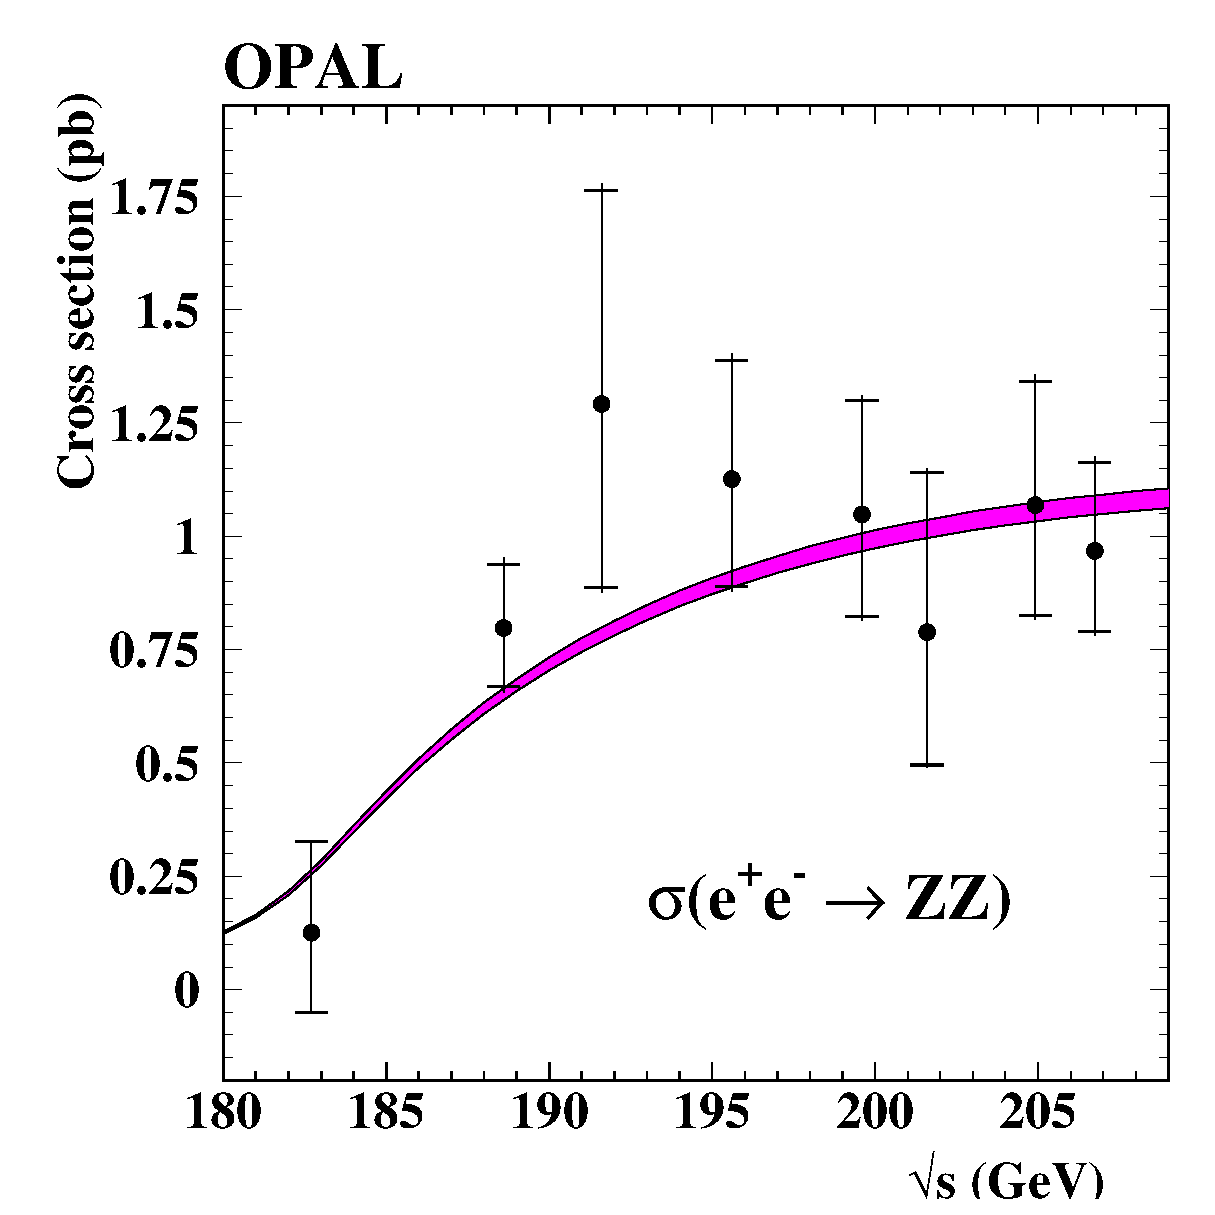
\includegraphics[width=0.7\textwidth]{phenomenology/OPAL_ZZxSec.eps}
    \caption[Measured $\epem \to \ZZ$ cross sections from OPAL.]{
        Measured $\epem \to \ZZ$ cross sections from the OPAL experiment, reproduced from Ref.~\cite{Abbiendi:2003va}.
        Points represent the measured values.
        Vertical bars are the total uncertainty with horizontal bars indicating the statistical uncertainties, which dominate.
        The band is the SM prediction with a 2\% theoretical uncertainty.
      }\label{fig:opalXSec}
  \end{center}
\end{figure}

Production in hadron collisions was first observed by the CDF and D0 experiments, in {1.96\TeV} {\ppb} events at Tevatron~\cite{Aaltonen:2008mv,Abazov:2008yf,Abazov:2008gya, Abazov:2011td,CDF:2011ab}.
In contrast to the LEP measurements, {\ppb} colliders cause too many extraneous jets for the hadronic channels to be seen above the background, so only the $4\ell$ and $2\ell2\Pnu$ ($\ell = \Pe, \Pm$) final states were used.
These fully leptonic decay modes have small branching fractions on top of the small {\ZZ} cross section of around {1.6\unit{pb}}~\cite{Campbell:1999ah}, but the total Tevatron dataset of roughly {6\fbinv} was large enough for CDF and D0 to find a few dozen events each.
Results were again fully consistent with the SM but the statistical uncertainties were large, as can be seen in the example $m_{4\ell}$ shown in Fig.~\ref{fig:D0m4l}~\cite{Abazov:2011td}.

\begin{figure}[htbp]
  \begin{center}
    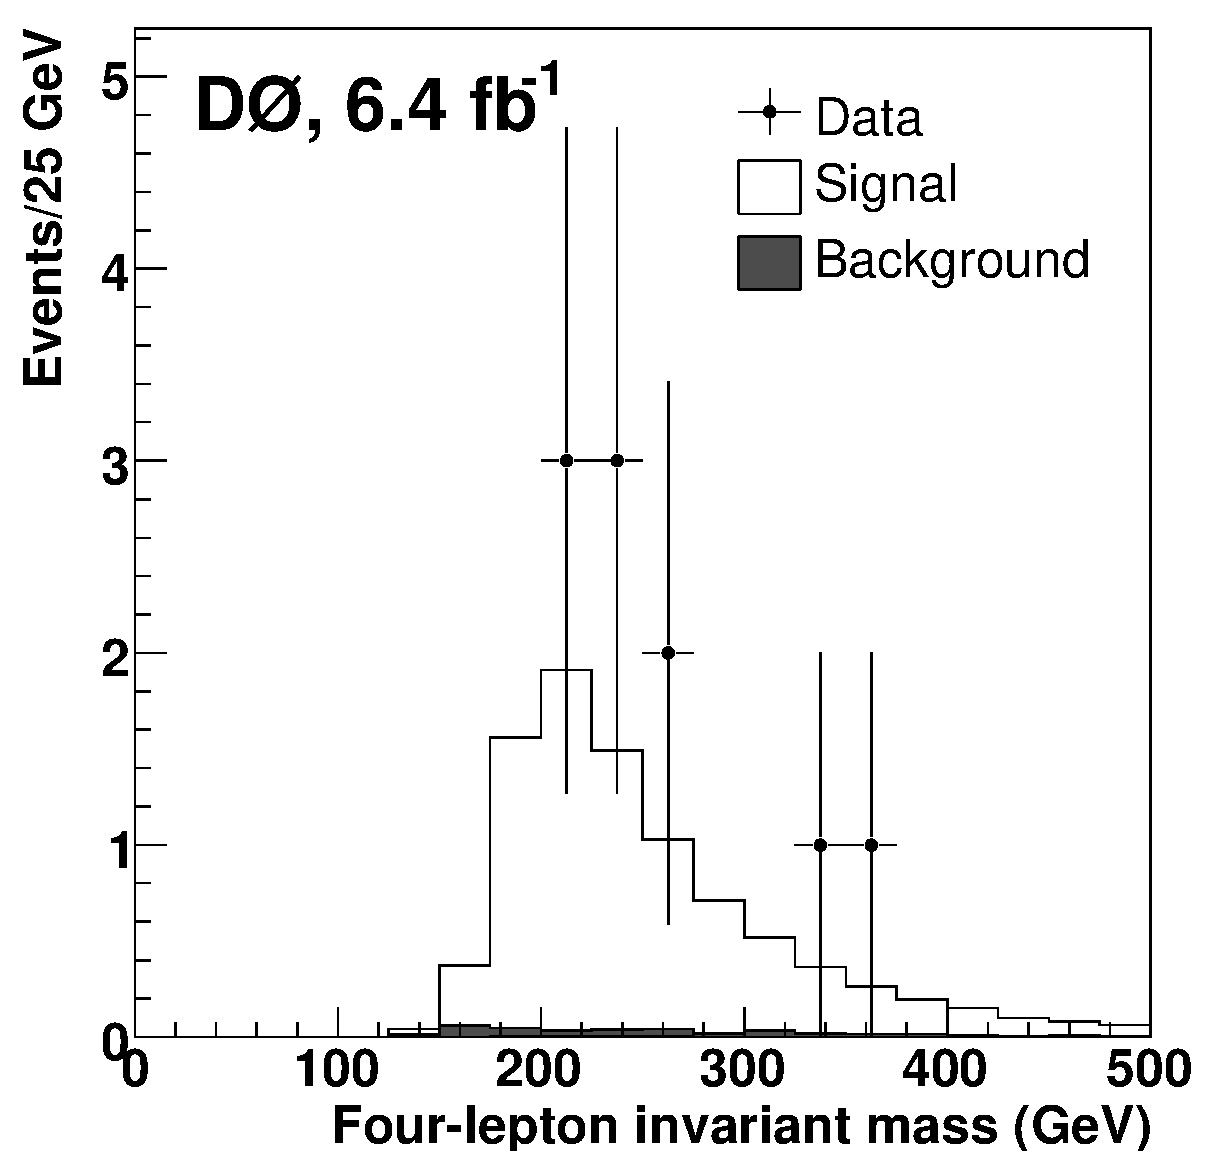
\includegraphics[width=0.7\textwidth]{phenomenology/D0m4l.eps}
    \caption[Measured four-lepton mass spectrum from D0.]{
        Measured $m_{4\ell}$ distribution from {\ZZ} events collected by D0, reproduced from Ref.~\cite{Abazov:2011td}.
        Points represent data with vertical bars showing statistical uncertainties, while the histograms show the SM expectation.
      }\label{fig:D0m4l}
  \end{center}
\end{figure}

The first run of the LHC (see Section~\ref{sec:lhc}) produced large datasets of {\pp} collisions at $\sqrt{s} = 7$ and {8\TeV}, producing {\ZZ} events with a higher cross section than at Tevatron~\cite{Cascioli:2014yka} and with a greater integrated luminosity.
The primary measurement channels were again the fully leptonic $4\ell$ and $2\ell2\Pnu$ decays, and the cross sections were measured at $\sqrt{s} = 7$ and {8\TeV} by both CMS~\cite{Chatrchyan:2012sga,CMS:2014xja,Khachatryan:2015pba, CMS-PAS-SMP-15-012} and ATLAS~\cite{Aad:2012awa,Aad:2015rka,Aaboud:2016urj}.
With a dataset of roughly {20\fbinv} and signal event counts in the hundreds even for the low-rate $4\ell$ channel, the {8\TeV} measurements had the statistical power to include differential cross sections as functions of kinematic observables for the {\ZZ} system and the associated jets.
Statistical uncertainties were still larger than the systematic uncertainties, but they were at the level of 5--10\% for the total cross section, compared to 30--50\% at Tevatron and 15--150\% at LEP depending on the experiment and center-of-mass energy\footnote{Most LEP {\ZZ} cross section measurements had statistical uncertainties around 20--40\%; see references given in the text for details.}.
The four-lepton mass spectra from the CMS and ATLAS {\ZZ} cross section measurements at {8\TeV} are shown in Figs.~\ref{fig:cms8TeVm4l} and~\ref{fig:atlas8TeVm4l}, respectively~\cite{CMS:2014xja,Aad:2015rka}.
A measurement was also performed on CMS data in the $\ZZ \to \lplm\Pqb\Paqb$ and $\ZZ \to \Pnu\Panu\Pqb\Paqb$ channels~\cite{Chatrchyan:2014aqa}.

\begin{figure}[htbp]
  \begin{center}
    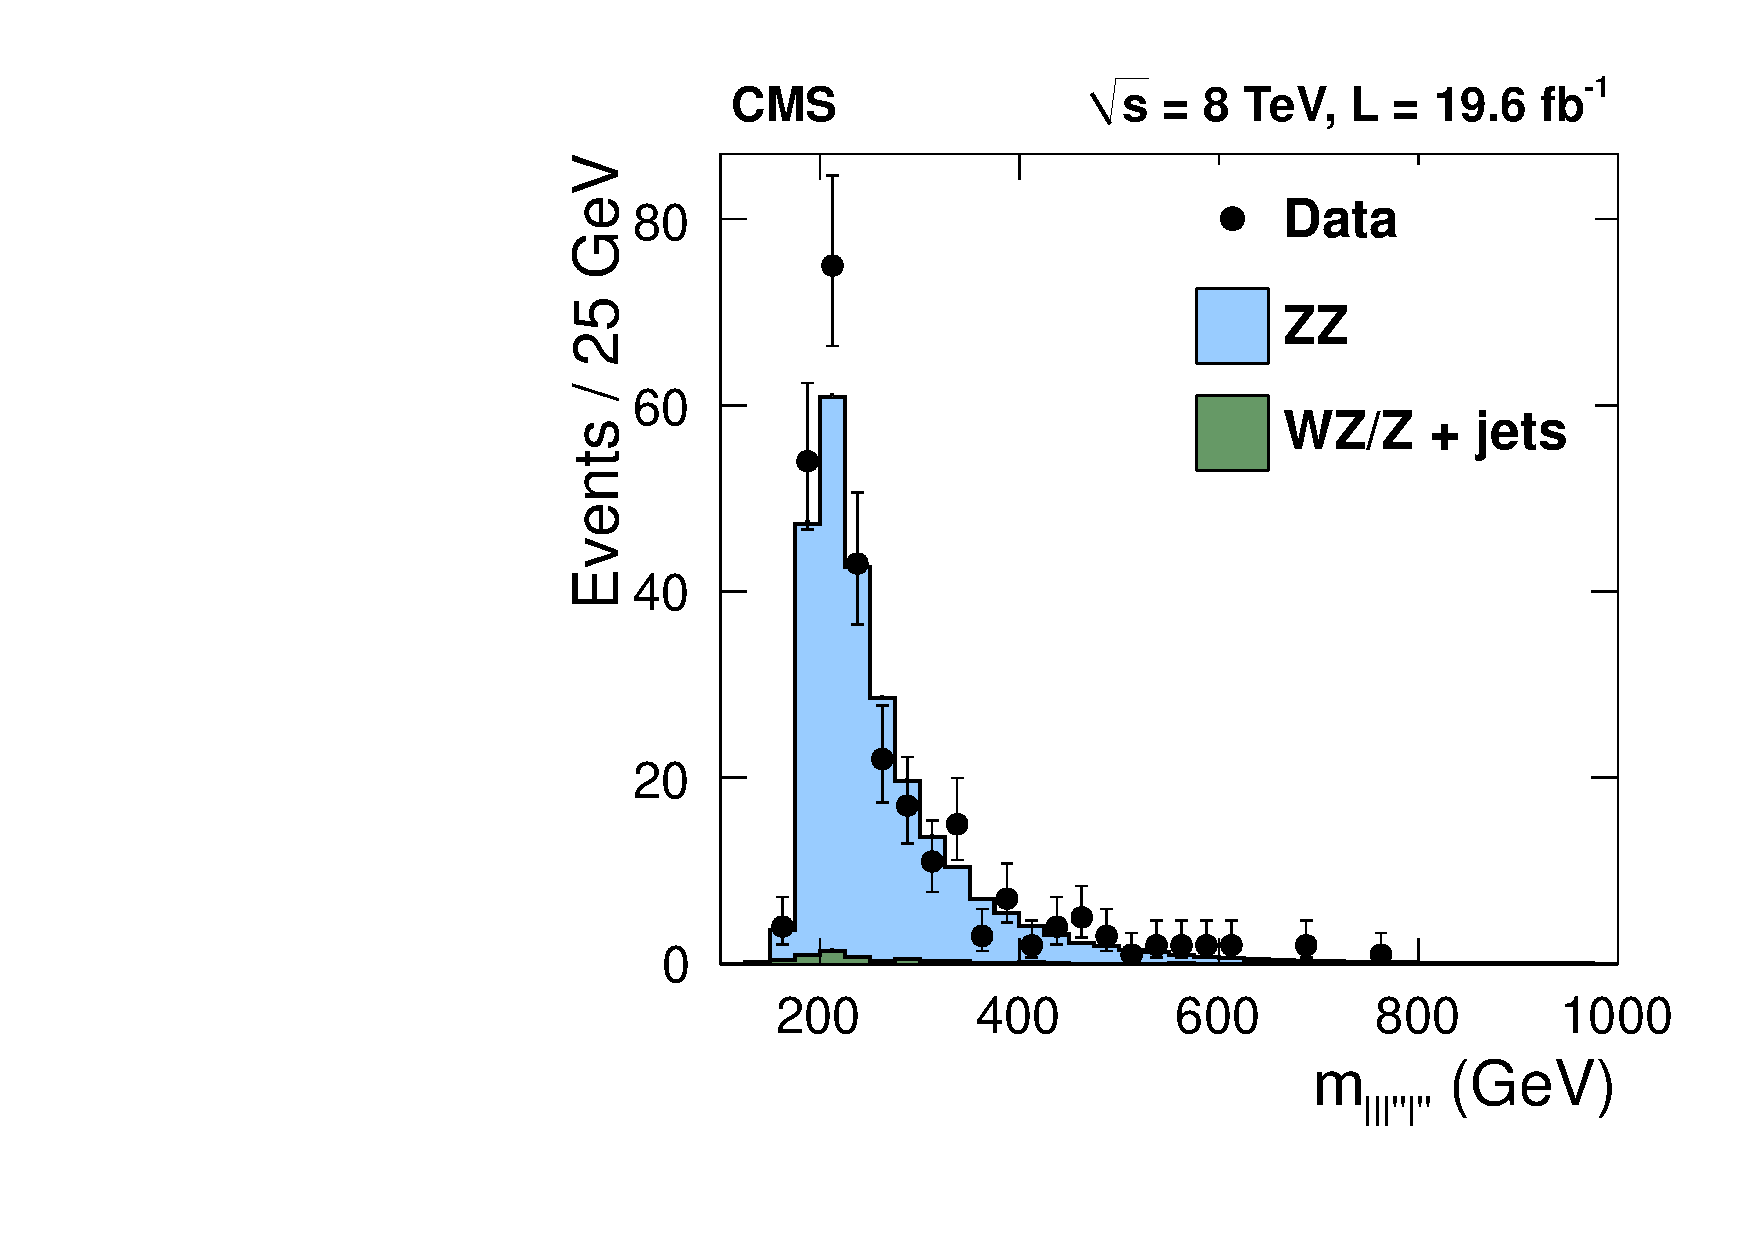
\includegraphics[width=0.7\textwidth]{phenomenology/CMS-SMP-13-005_Figure_002-a.pdf} % chktex 8
    \caption[Measured four-lepton mass spectrum from CMS at $\sqrt{s} = 8\TeV$.]{
        Measured $m_{4\ell}$ distribution from {\ZZ} events collected by CMS at $\sqrt{s} = 8\TeV$, reproduced from Ref.~\cite{Aad:2015rka}.
        Points represent data with vertical bars showing statistical uncertainties, while the histograms show the SM expectation.
        The grey hatched band represents the total uncertainty on the prediction.
      }\label{fig:cms8TeVm4l}
  \end{center}
\end{figure}

\begin{figure}[htbp]
  \begin{center}
    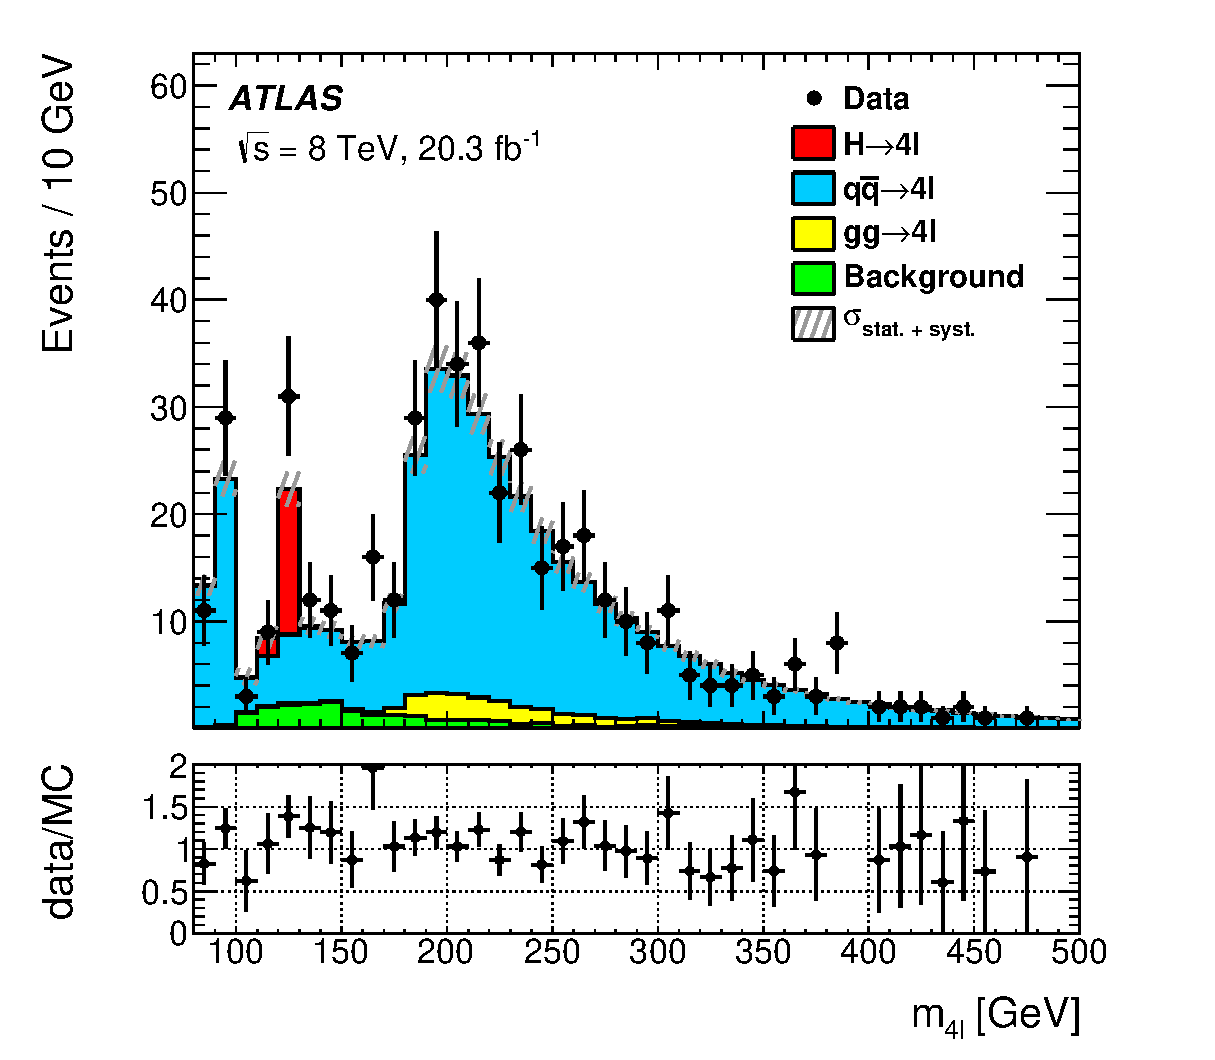
\includegraphics[width=0.7\textwidth]{phenomenology/ATLASm4l.eps}
    \caption[Measured four-lepton mass spectrum from ATLAS at $\sqrt{s} = 8\TeV$.]{
        Measured $m_{4\ell}$ distribution from {\ZZ} events collected by ATLAS at $\sqrt{s} = 8\TeV$, reproduced from Ref.~\cite{Abazov:2011td}.
        Points represent data with vertical bars showing statistical uncertainties, while the histograms show the SM expectation.
      }\label{fig:atlas8TeVm4l}
  \end{center}
\end{figure}

CMS found that the total {\ZZ} cross sections, defined as the cross sections of all events with two {\PZ} bosons in the mass range {60--120\GeV}, to be
\begin{equation}
  \begin{aligned}
    \sigma_{\ZZ}(7\TeV) & = 6.24 ^{+0.86}_{-0.80}\stat ^{+0.41}_{-0.32}\syst \pm 0.14\lum \unit{pb} \\
    \sigma_{\ZZ}(8\TeV) & = 7.7 \pm 0.5\stat ^{+0.5}_{-0.4}\syst \pm 0.4\thy \pm 0.2\lum \unit{pb},
  \end{aligned}
\end{equation}
when measured with $4\ell$ final states~\cite{Aad:2012awa,CMS:2014xja}, and
\begin{equation}
  \begin{aligned}
    \sigma_{\ZZ}(7\TeV) & = 5.1 ^{+1.5}_{-1.4}\stat ^{+1.4}_{-1.1}\syst \pm 0.1\lum \unit{pb} \\
    \sigma_{\ZZ}(8\TeV) & = 7.2 \pm 0.8\stat ^{+1.9}_{-1.5}\syst \pm 0.2\lum \unit{pb}
  \end{aligned}
\end{equation}
when measured with $2\ell2\Pnu$ final states~\cite{Khachatryan:2015pba}.
ATLAS found
\begin{equation}
  \begin{aligned}
    \sigma_{\ZZ}(7\TeV) & = 6.7 \pm 0.7\stat ^{+0.4}_{-0.3}\syst \pm 0.3\lum \unit{pb} \\
    \sigma_{\ZZ}(8\TeV) & = 7.3 \pm 0.4\stat \pm 0.3\syst \pm 0.2\lum \unit{pb},
  \end{aligned}
\end{equation}
using $4\ell$ final states at {7\TeV}~\cite{Aad:2012awa} and a combination of $4\ell$ and $2\ell2\Pnu$ events at {8\TeV}~\cite{Aaboud:2016urj}.
ATLAS used a slightly different definition of the {\PZ}, considering it to have mass in the range {66--116\GeV}, which reduces the SM expected cross section by 1.6\%~\cite{CMS:2017ruh}.
Measured cross sections from both experiments are again consistent with SM predictions of $6.7 \pm 0.2\unit{pb}$ at {7\TeV} and $8.3 \pm 0.2\unit{pb}$ at {8\TeV}, both calculated at NNNLO in QCD with \MATRIX, with factorization and renormalization scales $\mfmre m_\PZ$.

Searches for vector boson scattering were first performed at $\sqrt{s} = 8\TeV$.
The first process examined was the low-background same-sign {\WW} process $\pp \to \PWpm\PWpm\Pj\Pj$ studied at ATLAS, where evidence for electroweak production was observed at the level of a 3.6~standard deviation excess over the null hypothesis~\cite{Aad:2014zda}, and at CMS, where a $2.0\sigma$ excess was found~\cite{Khachatryan:2014sta}.
Subsequent searches for electroweak $\PZ\Pa\Pj\Pj$ production found a $3.0\sigma$ excess above the null hypothesis at CMS~\cite{Khachatryan:2017jub} and no significant excess at ATLAS~\cite{Aaboud:2017pds}.
A CMS measurement of $\PW\Pa\Pj\Pj$ production found a $2.7\sigma$ excess above the null hypothesis consistent with electroweak production~\cite{Khachatryan:2016vif}.
Searches for photon-photon VBS were performed as searches for exclusive and quasi-exclusive $\Pa\Pa \to \PWp\PWm$ production $\pp \to \Pp^{(\ast)}\PWp\PWm\Pp^{(\ast)}$, in which the protons do not collide but instead both radiate photons, which scatter.
CMS found evidence at the level of $3.4\sigma$ above the null hypothesis~\cite{Khachatryan:2016mud}, and ATLAS saw a $3.0\sigma$ excess~\cite{Aaboud:2016dkv}.
Roughly contemporaneously with this work, electroweak same-sign {\WW} production was observed at CMS in {13\TeV} collisions, with a significance of $5.5\sigma$~\cite{CMS-PAS-SMP-17-004}.
No searches for Electroweak {\ZZ} production had been performed prior to the analysis described in the following chapters.



\section[Resonant
         \texorpdfstring{$\mathrm{ZZ}^\ast$/$\mathrm{Z\gamma}^\ast$}
         {ZZ*/gamma*gamma*}
         Production]{Resonant $\mathbf{ZZ}^\ast$/$\gamma^\ast\gamma^\ast$ Production}

Resonant production appears as a sharp peak in the four-lepton invariant mass distribution over the broad spectrum from nonresonant production.
There are two known four-lepton resonances: single-{\PZ} decays to four leptons around {91\GeV}, and Higgs decays to {\ZZs} around {125\GeV}.
Another resonance, caused by a new particle, could still be discovered at high mass, or at low mass but with a very small cross section.


\subsection{Z Boson Decays to Four Leptons}

A single {\PZ} boson may decay to a four-lepton final state when a lepton from a normal $\PZ \to \lplm$ decay radiates a virtual photon, as shown in Fig~\ref{fig:z4lDiagram}.
In a window around the {\PZ} mass of $80 < m_{4\ell} < 100\GeV$, $t$- and $u$-channel production (the diagrams of Fig~\ref{fig:zzLO} with $\Pa^\ast$ for both bosons) contribute at the few-percent level (4\% at $\sqrt{s} = 13\TeV$).
Four-fermion decays were studied in detail at LEP~\cite{Buskulic:1994gk}.
This included four-lepton decays, but used all $\lplm\Pf\Paf (\ell = \Pe,\Pm,\Pt)$ final states, where {\Pf} could be any fermion except the neutrinos.
{\Zfourl} decays were also observed at 7 and~{8\TeV} at CMS, where the branching fraction was found to be $\mathcal{B}(\Zfourl) = 4.2 ^{+0.9}_{-0.8}\stat \pm 0.2\syst \times 10^{-6}$~\cite{CMS:2012bw}, and at ATLAS, where it was found to be $3.20 \pm 0.25\stat \pm 0.13\syst \times 10 ^{-6}$ in a slightly different phase space~\cite{Aad:2014wra}.
After correcting for phase space differences, the measurements are compatible with each other and with the SM\@.

\begin{figure}[htbp]
  \vspace{1em}
  \begin{center}
    \begin{fmffile}{z4l}
      \begin{fmfgraph*}(0.325,0.25) % chktex 36
        \fmfleft{d1,i1,d2}
        \fmfright{o1,o2,o3,o4}
        \fmflabel{\PZ}{i1}
        \fmflabel{\Plp}{o1}
        \fmflabel{\Plpp}{o2}
        \fmflabel{\Plpm}{o3}
        \fmflabel{\Plm}{o4}
        \fmf{zigzag,tension=3}{i1,v1}
        \fmf{phantom}{o1,v1,o4}
        \fmffreeze % chktex 1
        \fmf{fermion}{o1,v2,v1,o4}
        \fmf{boson,label={$\Pa^\ast$}}{v2,v3}
        \fmf{fermion}{o2,v3,o3}
      \end{fmfgraph*}
    \end{fmffile}
    \vspace{1em}
    \caption[Feynman diagram for {\Zfourl} production]{
      Tree-level Feynman diagram for {\Zfourl} production.
      Either initial lepton may radiate the $\Pa^\ast$.
      }\label{fig:z4lDiagram}
  \end{center}
\end{figure}


\subsection{Higgs Boson Production}\label{sec:Hproduction}

The primary Higgs production mechanism in multi-{\TeVns} hadron collisions is gluon-gluon fusion through a quark loop, because of the gluon's high effective luminosity and the top quark's strong Yukawa coupling.
Other mechanisms, in decreasing order by cross section, include vector boson fusion (VBF), vector boson associated production ({\VH} or ``Higgsstrahlung''), and top-antitop associated production ({\TTH}).
Tree-level Feynman diagrams for all four are shown in Fig.~\ref{fig:Hprod}.
The SM cross sections for the various production mechanisms, and the Higgs branching fractions, are shown as functions of $m_\PH$ near the measured mass of {125\GeV} in Fig.~\ref{fig:HxsecBR}.
Gluon-gluon fusion has roughly an order of magnitude higher rate than the others.
The VBF process contributes to the unitarization of vector boson scattering along with the diagrams in Fig.~\ref{fig:vbs}.
Decays to {\ZZs} are heavily suppressed by the fact that, since $m_\PH < 2m_\PZ$, energy conservation requires one of the {\PZ} bosons to be far off its mass shell.
Decays to four charged leptons are further suppressed by the small $\PZ \to \lplm$ branching fraction.
However, the distinctive signature of four high-energy charged leptons in a single event is easy to detect with high efficiency and background rejection, and the momentum of electrons and muons can in general be measured with high precision, allowing the Higgs resonance to be easily seen as a sharp peak over a small, relatively flat background, and $\PH \to 4\ell$ is one of the most attractive channels for Higgs discovery and measurement of its properties.

\begin{figure}[htbp]
  \vspace{1em}
  \begin{center}
    \begin{fmffile}{ggH}
      \begin{fmfgraph*}(0.3,0.25) % chktex 36
        \fmfstraight %chktex 1
        \fmfleft{i1,d1,d2,i2}
        \fmfright{o1,o2,o3,o4}
        \fmflabel{\Pg}{i1}
        \fmflabel{\Pg}{i2}
        \fmflabel{\Plp}{o3}
        \fmflabel{\Plm}{o4}
        \fmflabel{\Plpp}{o1}
        \fmflabel{\Plpm}{o2}
        \fmf{fermion}{v1,v2,v3,v1}
        \fmf{dashes,label={\PH},tension=1.8}{v3,v4}
        \fmf{zigzag,label={\PZ},tension=1.4}{v4,v6}
        \fmf{zigzag,label={$\PZ^\ast$},tension=1.4}{v4,v5}
        \fmf{fermion}{o1,v5,o2}
        \fmf{fermion}{o3,v6,o4}
        \fmf{gluon,tension=1.8}{i1,v1}
        \fmf{gluon,tension=1.8}{i2,v2}
        % phantoms to make a phantom vertex to label
        \fmf{phantom}{v1,v7}
        \fmf{phantom}{v2,v7}
        \fmf{phantom}{v3,v7}
        \fmfv{label={\Pqt},l.d=0}{v7}
      \end{fmfgraph*}
    \end{fmffile}
    \hspace{4em}
    \begin{fmffile}{vbfH}
      \begin{fmfgraph*}(0.3,0.25) % chktex 36
        \fmfstraight %chktex 1
        \fmfleft{i1,d1,d2,i2}
        \fmfright{o1,o2,o3,o4,o5,o6}
        \fmflabel{$\Pq_1$}{i1}
        \fmflabel{$\Pq_2$}{i2}
        \fmflabel{$\Pq_1^\prime$}{o1}
        \fmflabel{$\Pq_2^\prime$}{o6}
        \fmflabel{\Plpp}{o2}
        \fmflabel{\Plpm}{o3}
        \fmflabel{\Plp}{o4}
        \fmflabel{\Plm}{o5}
        \fmf{fermion}{i1,v1,o1}
        \fmf{phantom}{d1,v1}
        \fmf{phantom}{d2,v3}
        \fmf{phantom}{v1,v4,v5,v3}
        \fmf{fermion}{i2,v3,o6}
        \fmffreeze % chktex 1
        \fmf{zigzag,label={\PWmp,,\PZ},tension=1.3,l.s=left}{v1,v2}
        \fmf{zigzag,label={\PWpm,,\PZ},tension=1.3,l.s=left}{v2,v3}
        \fmf{dashes,label={\PH}}{v2,v8}
        \fmf{zigzag,label={$\PZ^\ast$},l.s=right}{v8,v6}
        \fmf{zigzag,label={\PZ},l.s=left}{v8,v7}
        \fmf{fermion}{o2,v6,o3}
        \fmf{fermion}{o4,v7,o5}
      \end{fmfgraph*}
    \end{fmffile}
    \vspace{4em}

    \begin{fmffile}{vH}
      \begin{fmfgraph*}(0.3,0.25) % chktex 36
        \fmfstraight %chktex 1
        \fmfleft{d1,i1,i2,d2}
        \fmfright{o1,d3,o2,o3,o4,o5}
        \fmflabel{\Pq}{i1}
        \fmflabel{\Paq}{i2}
        \fmflabel{{$\PWpm,\PZ$}}{o1}
        \fmflabel{\Plpp}{o2}
        \fmflabel{\Plpm}{o3}
        \fmflabel{\Plp}{o4}
        \fmflabel{\Plm}{o5}
        \fmf{fermion}{i1,v1,i2}
        \fmf{zigzag}{v1,v2}
        \fmf{phantom}{d1,v2,d2}
        \fmf{phantom}{o1,v2,o5}
        \fmffreeze % chktex 1
        \fmf{zigzag}{v2,o1}
        \fmf{dashes,label={\PH},label.side=left}{v2,v3}
        \fmf{zigzag,label={\PZ},l.s=left}{v3,v4}
        \fmf{zigzag,label={$\PZ^\ast$},l.s=right}{v3,v5}
        \fmf{fermion}{o2,v5,o3}
        \fmf{fermion}{o4,v4,o5}
      \end{fmfgraph*}
    \end{fmffile}
    \hspace{4em}
    \begin{fmffile}{ttH}
      \begin{fmfgraph*}(0.3,0.25) % chktex 36
        \fmfstraight %chktex 1
        \fmfleft{d1,i1,d2,d3,i2,d4}
        \fmfright{o1,o2,o3,o4,o5,o6}
        \fmflabel{\Pg}{i1}
        \fmflabel{\Pg}{i2}
        \fmflabel{\Paqt}{o1}
        \fmflabel{\Pqt}{o6}
        \fmflabel{\Plpp}{o2}
        \fmflabel{\Plpm}{o3}
        \fmflabel{\Plp}{o4}
        \fmflabel{\Plm}{o5}
        \fmf{fermion}{o1,v1,v2,v3,o6}
        \fmf{gluon}{i1,v1}
        \fmf{gluon}{i2,v3}
        \fmf{dashes,label={\PH}}{v2,v4}
        \fmf{zigzag,label={$\PZ^\ast$},l.s=right}{v4,v5}
        \fmf{zigzag,label={\PZ},l.s=left}{v4,v6}
        \fmf{fermion}{o2,v5,o3}
        \fmf{fermion}{o4,v6,o5}
        \fmf{phantom}{d1,v1,d2}
        \fmf{phantom}{d3,v3,d4}
      \end{fmfgraph*}
    \end{fmffile}
    \vspace{1em}
    \caption[Higgs production mechanisms]{
      Tree-level Higgs production diagrams for gluon-gluon fusion (top left), VBF (top right), {\VH} (bottom left), and {\TTH}, decaying to four leptons.
      }\label{fig:Hprod}
  \end{center}
\end{figure}

\begin{figure}[htbp]
  \begin{center}
    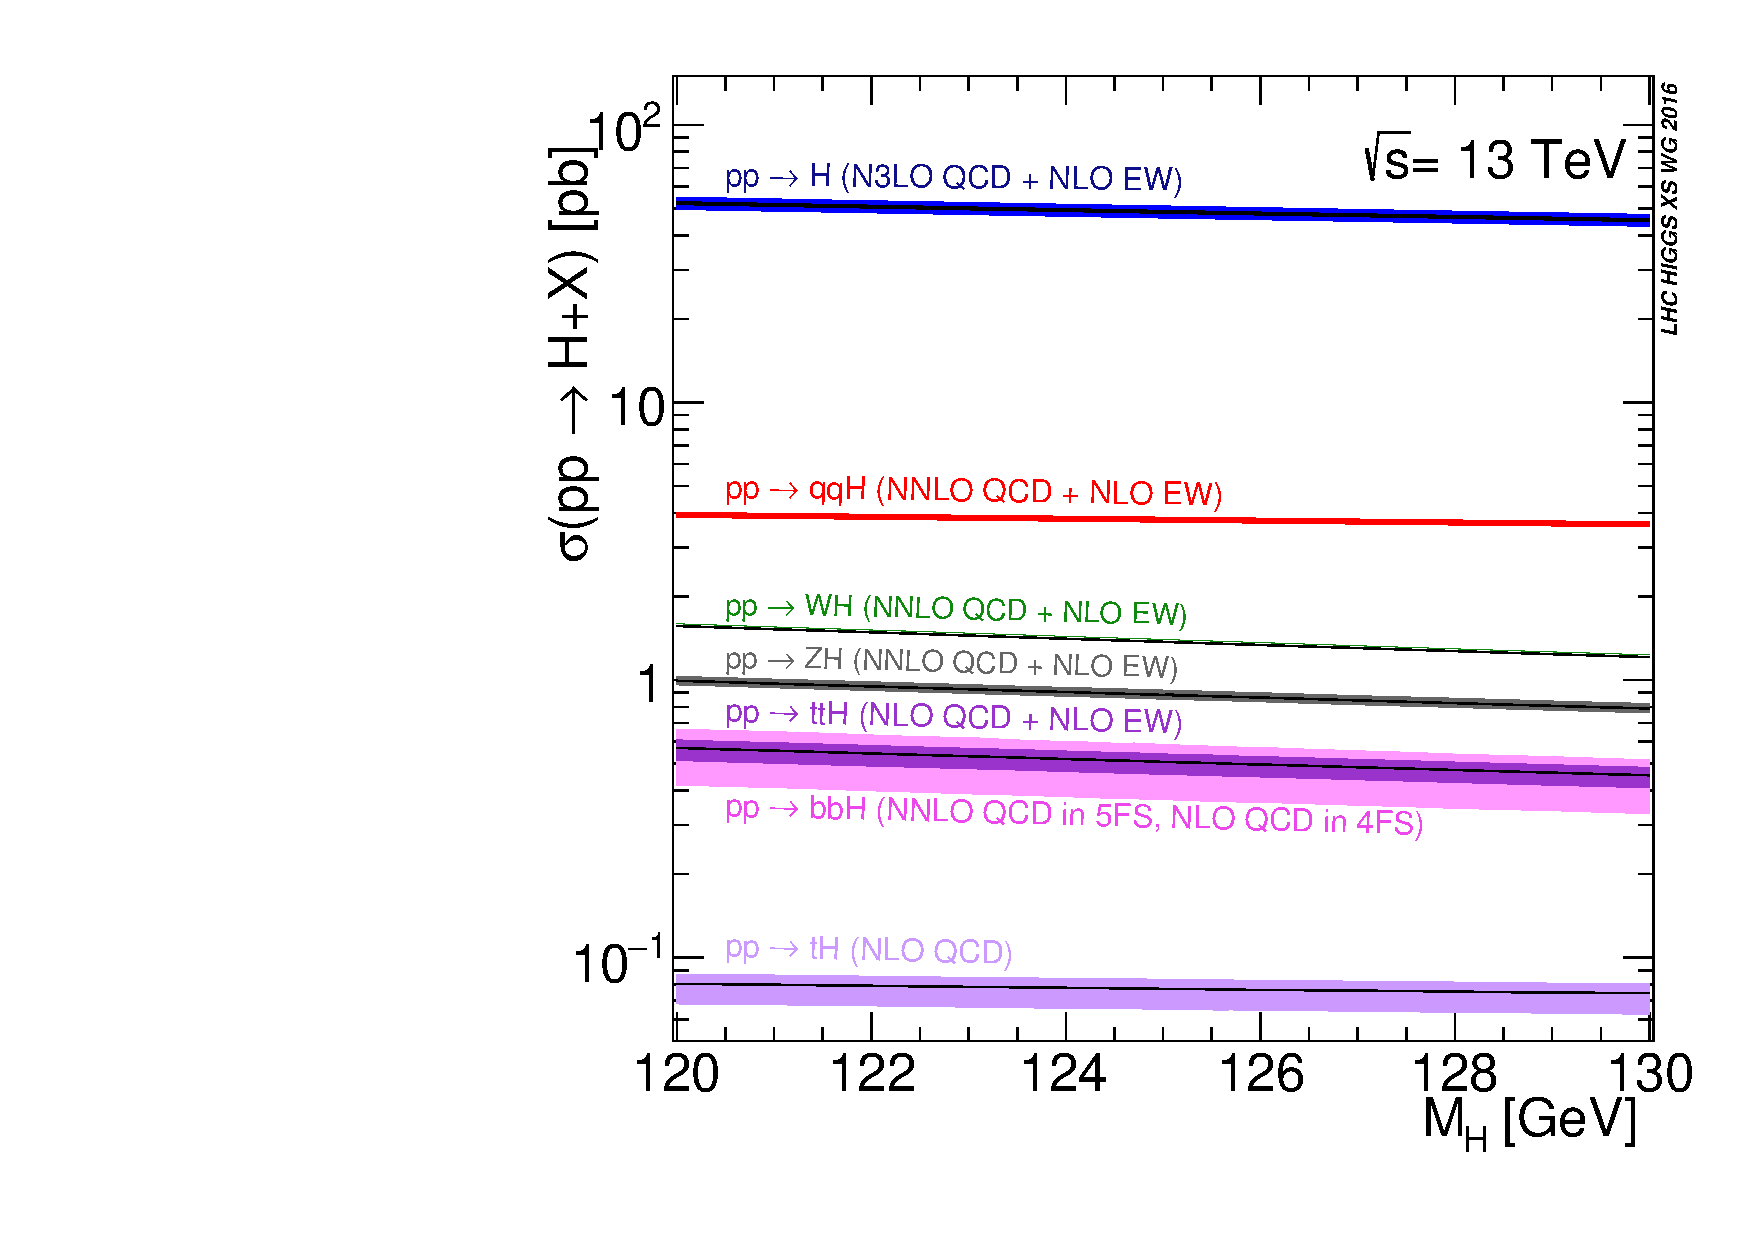
\includegraphics[width=0.48\textwidth]{phenomenology/plot_13tev_H_sqrt.pdf}
    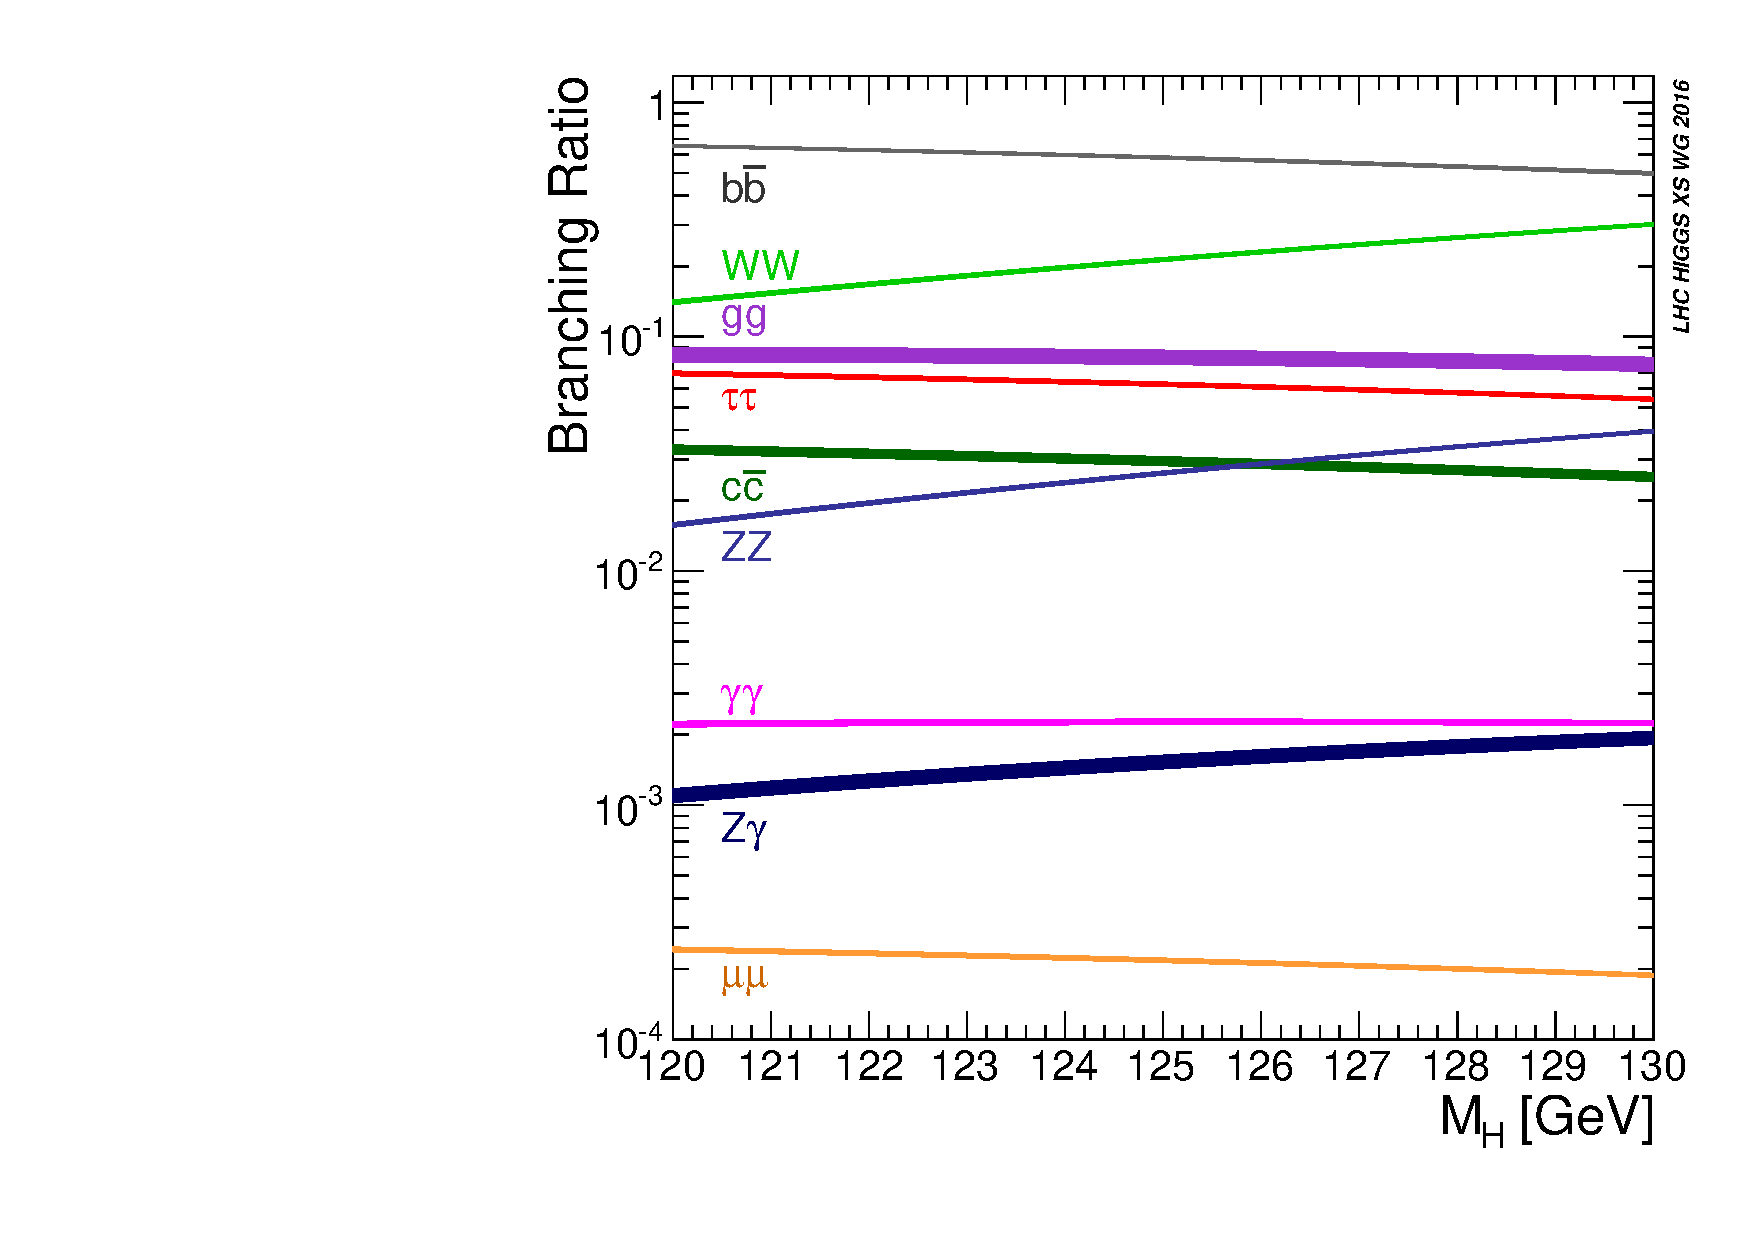
\includegraphics[width=0.48\textwidth]{phenomenology/SMHiggsBR_YR4-square.pdf}
    \caption[Higgs boson SM cross section and branching ratio, as a function of $m_\PH$]{
        The SM cross sections for each Higgs boson production mode (left) and the Higgs branching fraction to several important final states (right), as a function of Higgs mass near the measured mass of {125\GeV}.
        Both plots are reproduced from Ref.~\cite{deFlorian:2016spz}.
      }\label{fig:HxsecBR}
  \end{center}
\end{figure}

\subsubsection{Prior Measurements}\label{sec:Hresults}

Higgs boson searches at LEP were for {\PZ}-associated production, which has the highest cross section in {\epem} collisions.
The maximum LEP center-of-mass energy, {209\GeV}, was just under the {\ZH} threshold around {216\GeV}.
The LEP combined 95\% confidence level (CL) lower limit on $m_\PH$ was {114.4\GeV}~\cite{Barate:2003sz}, and a combination of LEP data and electroweak precision measurements set an upper limit of {193\GeV}~\cite{Alcaraz:2006mx}.
Searches at the CDF and D0 experiments at the Tevatron were combined to find a $3.0\sigma$ local excess ($2.8\sigma$ global) consistent with $m_\PH = 125\GeV$~\cite{Aaltonen:2013ioz}, with the $\PH \to \Pqb\Paqb$ search alone finding a local excess of $3.3\sigma$ ($3.1\sigma$ local)~\cite{Aaltonen:2012qt}.
Results from all the Tevatron and LEP measurements and electroweak precision measurements were combined to place an upper mass limit of {158\GeV} at 95\% CL~\cite{ALEPH:2010aa}.
The Higgs was finally discovered simultaneously by the CMS and ATLAS collaborations with a combination of 7~and~{8\TeV} data~\cite{Chatrchyan:2012xdj,Aad:2012tfa}.
The four-lepton channel was, as anticipated, one of the most important~\cite{Chatrchyan:2012dg,Chatrchyan:2012xdj}.
Its properties were subsequently investigated in detail at both experiments.
The Higgs mass was found to be
\begin{equation}
  m_\PH = 125.09 \pm 0.21\stat \pm 0.11\syst \GeV
\end{equation}
based on a combination of data from the two experiments~\cite{Aad:2015zhl}, and SM predictions of its properties have been confirmed by a number of measurements~\cite{Khachatryan:2016vau}.


\section{Anomalous Gauge Couplings}

A primary hallmark of anomalous couplings is an enhanced cross section at center-of-mass energies of order {1\TeV}~\cite{Baur:2000ae}.
The increase in cross section at high $m_{4\ell}$ implies higher transverse momentum for the outgoing {\PZ} bosons and leptons, as shown for two example aTGC models in Fig.~\ref{fig:aTGCxsecChange}.
Searches for high-mass {\ZZ} events are attractive because SM continuum production cross sections are extremely small above a few hundred {\GeVns} and all other sources of prompt or nonprompt four-lepton events are negligible, so even a handful of events would be an unambiguous sign of new physics.
The search for nonzero aTGCs is performed using inclusive {\ZZ} events, because the aTGC parameters should not have a large effect on jet distributions.
The aQGC search is performed in {\ZZjj} events because it would specifically enhance the VBS cross section at high mass.

\begin{figure}[htbp]
  \begin{center}
    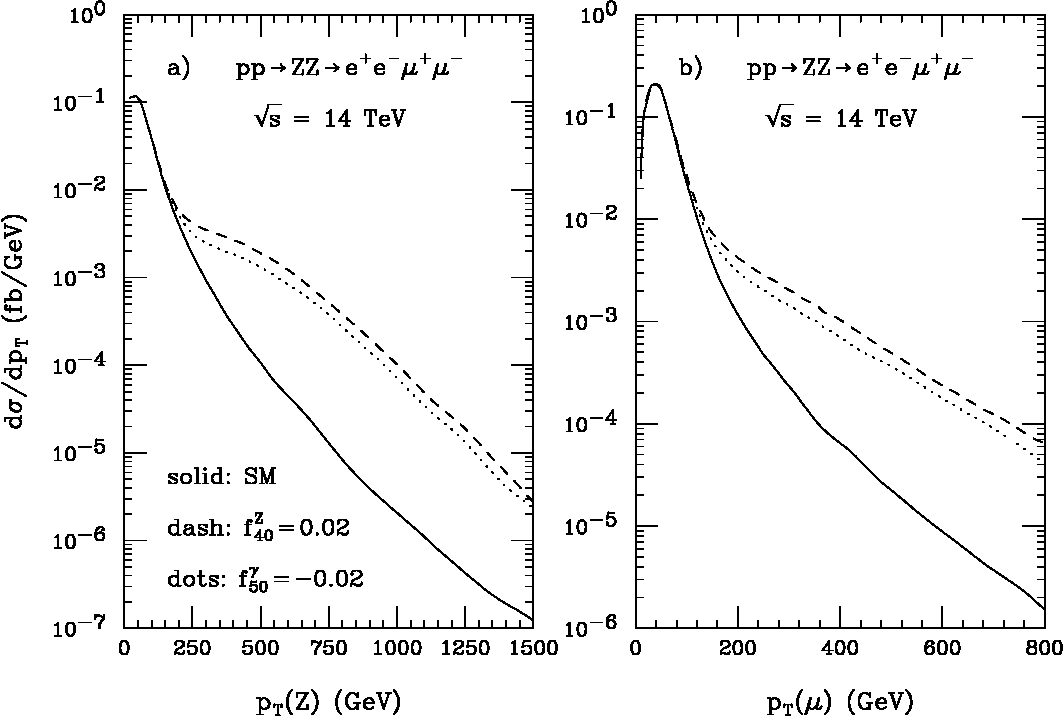
\includegraphics[width=0.9\textwidth]{phenomenology/pt_lhc_4l.pdf}
    \caption[Enhancements in $\pt^\PZ$ and $\pt^\Pm$ resulting from nonzero aTGCs]{
        Cross section enhancements at high {\PZ} and {\Pm} momenta caused by example nonzero aTGCs.
        Reproduced from Ref.~\cite{Baur:2000ae}.
      }\label{fig:aTGCxsecChange}
  \end{center}
\end{figure}

The neutral aTGC parameters $f_4^\PV$ and $f_5^\PV$ are expected to have almost identical effects at high energy, so the search variables cannot be used to determine the relative strengths of the possible anomalous couplings~\cite{Baur:2000ae}.
However, because the terms governed by $f_4^\PV$ have opposite behavior to the terms governed by $f_5^\PZ$ under parity transformations, they affect the helicity amplitudes of the {\PZ} bosons and alter the angular distributions of the final-state leptons.
Figure~\ref{fig:aTGCangles} shows the cross section as a function of total angular distance and the azimuthal angular difference between muons from the same {\PZ} decay for several example nonzero aTGCs and for the SM\@.
These distributions could be used to distinguish between the possible aTGC parameters and determine the sign of the CP-conserving $f_5^\PV$ terms.

\begin{figure}[htbp]
  \begin{center}
    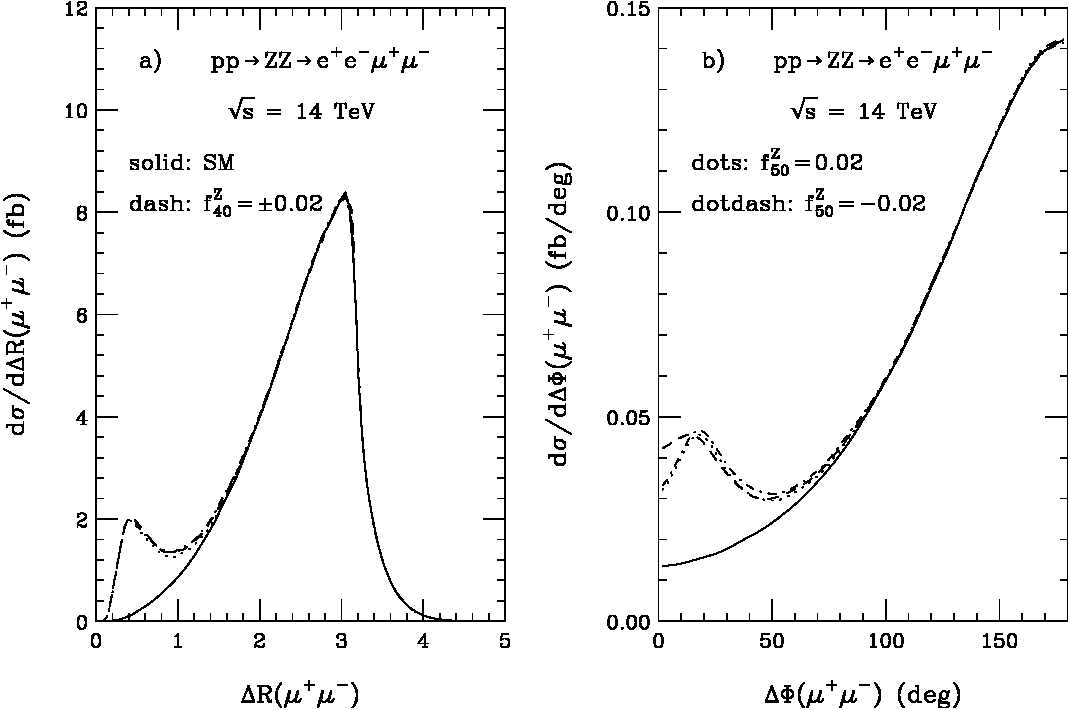
\includegraphics[width=0.9\textwidth]{phenomenology/r_phi_lhc_4l.pdf}
    \caption[Lepton angular correlations resulting from nonzero aTGCs]{
        Total angular distance and azimuthal angular difference between muons from the same the same {\PZ} decay caused by several example nonzero aTGCs.
        Reproduced from Ref.~\cite{Baur:2000ae}.
      }\label{fig:aTGCangles}
  \end{center}
\end{figure}



\subsection{Previous Limits}\label{sec:aTGCLit}

The first neutral aTGC searches were performed at LEP using {\ZZ} and {$\PZ\Pa$} events~\cite{Abbiendi:2003va,Ots:2004hk, Abdallah:2007ae,Schael:2009zz}.
Depending on the experiment and parameter, 95\% CL limits were generally $\mathcal{O}(\pm1)$, and the statistical combination set limits around 0.2--0.4~\cite{Alcaraz:2006mx}.
The first searches in hadron collisions were performed at Tevatron the by CDF collaboration, which set symmetric 95\% CL limits in the range $\pm 0.10$--0.13 for all parameters~\cite{Robson:2012np}, and the D0 collaboration, which set symmetric limits around $\pm0.20$--0.31 for all parameters~\cite{Abazov:2007ad}.
Both Tevatron experiments used a unitarity-preserving cutoff of $\Lambda = 1.2\TeV$.
CMS and ATLAS set 95\% CL limits at {7\TeV} at $\mathcal{O}(\pm0.1)$~\cite{Chatrchyan:2012sga,Aad:2011xj,Aad:2012awa}, and $\mathcal{O}(\pm0.005)$ at {8\TeV}~\cite{CMS:2014xja,Aad:2015zqe}.
ATLAS presented limits from {7\TeV} data with and without a unitarizing form factor; their {8\TeV} results, and all CMS results, did not use one.
Prior to this work, the most stringent limits on all four neutral aTGC parameters were set by CMS with a combination of 7~and {8\TeV} data~\cite{Khachatryan:2015pba},
\begin{equation}\label{eq:aTGC1DPrevious}
  \begin{aligned}
  & -0.0022 < f_4^\PZ < 0.0026   ,  & -0.0023 < f_5^\PZ < 0.0023 , \\
  & -0.0029 < f_4^\Pa < 0.0026   ,  & -0.0026 < f_5^\Pa < 0.0027 .
  \end{aligned}
\end{equation}
The two-dimensional aTGC limits set by CMS with the {8\TeV} dataset are shown in Fig.~\ref{fig:cms8TeVaTGC}~\cite{CMS:2014xja}.

\begin{figure}[htbp]
  \begin{center}
    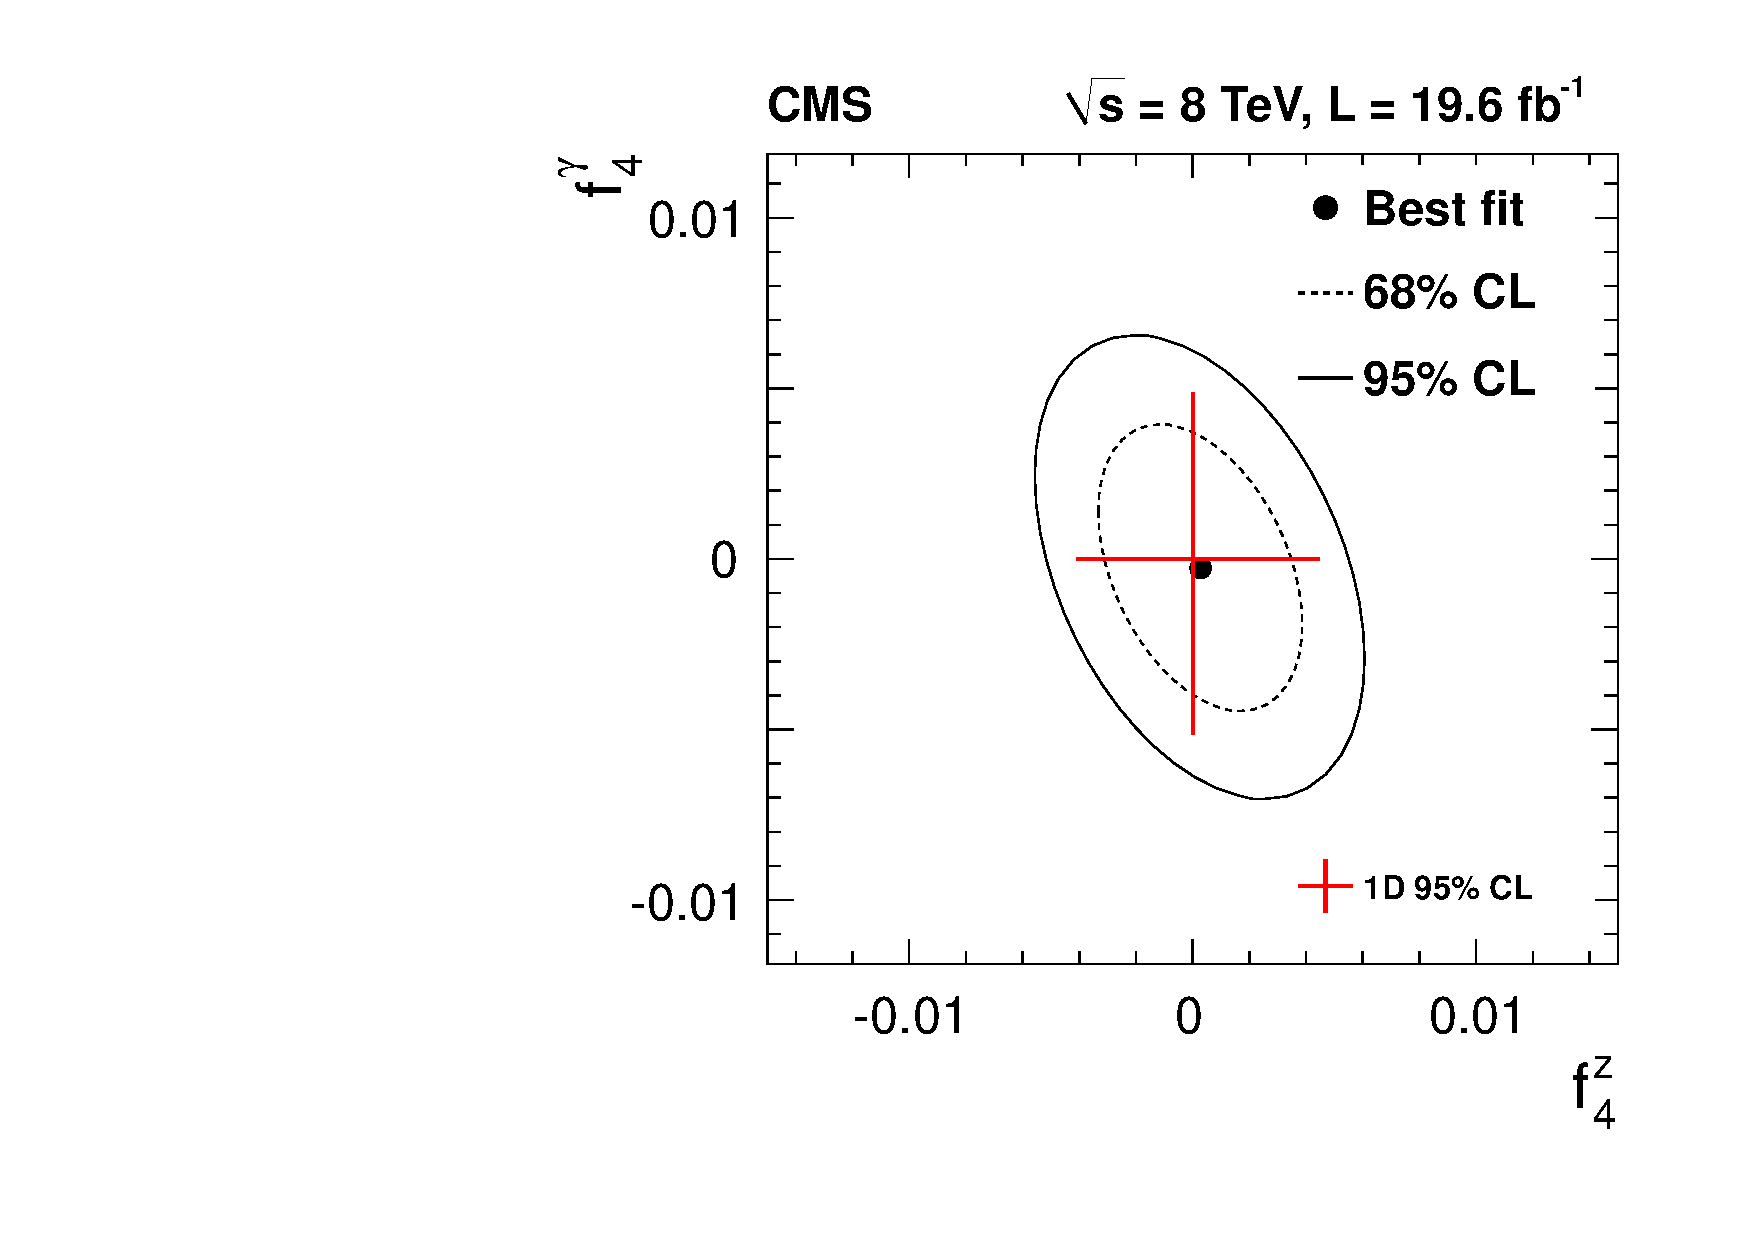
\includegraphics[width=0.48\textwidth]{phenomenology/CMS-SMP-13-005_Figure_006-a.pdf} % chktex 8
    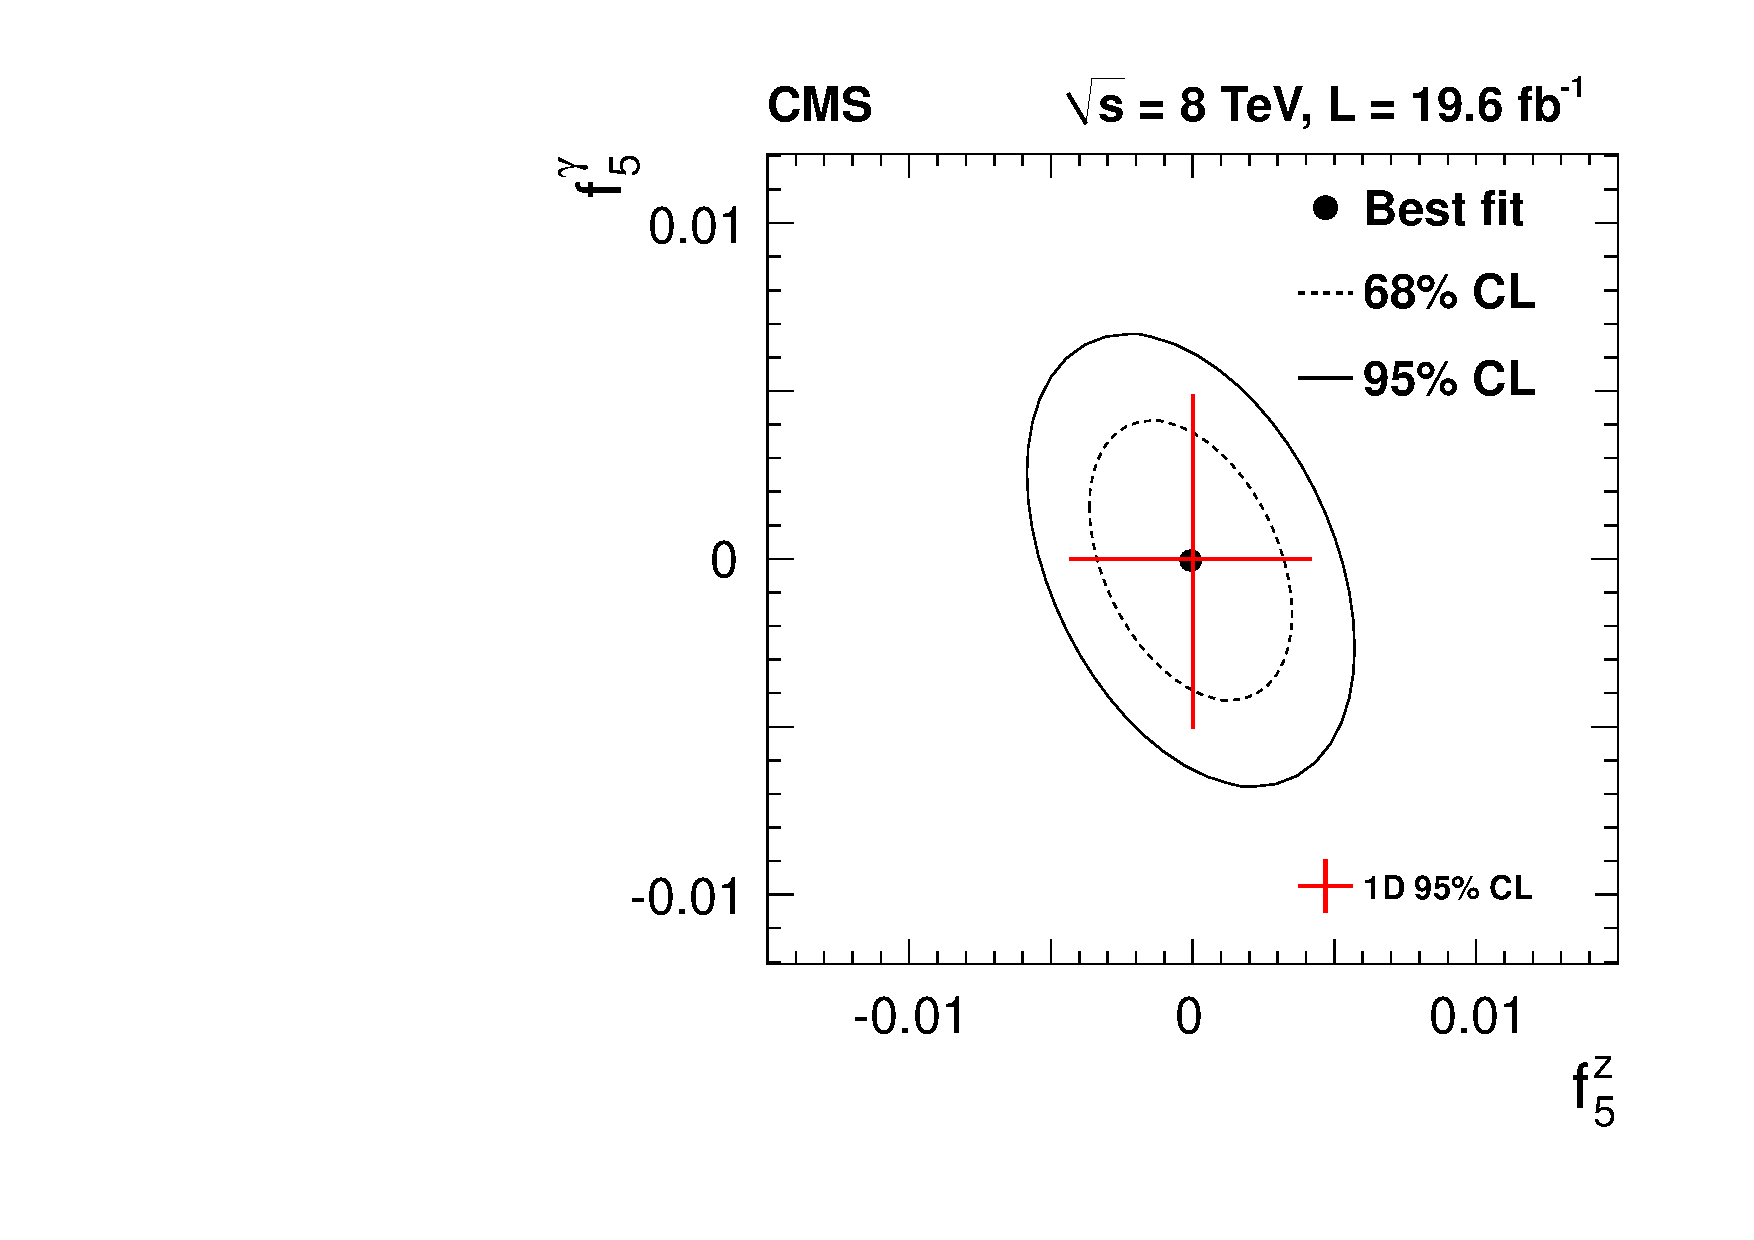
\includegraphics[width=0.48\textwidth]{phenomenology/CMS-SMP-13-005_Figure_006-b.pdf} % chktex 8
    \caption[Previous two-dimensional aTGC limits from CMS.]{
        Two-dimensional 95\% CL aTGC limits set by CMS, reproduced from Ref.~\cite{CMS:2014xja}.
      }\label{fig:cms8TeVaTGC}
  \end{center}
\end{figure}

No prior aQGC searches were performed using {\ZZ} processes, but both LHC experiments set limits on the {\ZZ}-sensitive effective field theory operators using other channels.
The most stringent limits on $f_\text{T0}$ were from $\sqrt{s} = 8\TeV$ $\PZ\Pa\Pq\Pq$ events at ATLAS~\cite{Aaboud:2017pds}, found to be
\begin{equation}
  -3.4 < f_\text{T0} / \Lambda^4 < 2.9 \TeV^{-4}
\end{equation}
at 95\% CL, with similar results produced by CMS~\cite{Khachatryan:2017jub}.
The most stringent limits on $f_\text{T1}$ and $f_\text{T2}$ were set by CMS at {8\TeV} using same-sign {$\WW\Pq\Pq$} events~\cite{Khachatryan:2014sta}, and were found to be
\begin{equation}
  -2.1 < f_\text{T1} / \Lambda^4 < 2.4 \TeV^{-4}
\end{equation}
and
\begin{equation}
  -5.9 < f_\text{T2} / \Lambda^4 < 7.1 \TeV^{-4}.
\end{equation}
CMS and ATLAS produced nearly identical limits on $f_\text{T8}$ and $f_\text{T9}$ in the same $\PZ\Pa\Pq\Pq$ searches that set limits on $f_\text{T0}$,
\begin{equation}
  -1.8 < f_\text{T8} / \Lambda^4 < 1.8 \TeV^{-4}
\end{equation}
and
\begin{equation}
  -3.9 < f_\text{T9} / \Lambda^4 < 3.9 \TeV^{-4}.
\end{equation}



\section{Background Processes}\label{sec:bkgPheno}

Spurious events are categorized as irreducible backgrounds, i.e.\ those that are expected to have four prompt leptons, and reducible backgrounds, which have two or three prompt leptons and another object that is misidentified as a prompt lepton.
The only nontrivial irreducible backgrounds to inclusive $\ZZ/\PZ\Pa^\ast$ production are {\WWZ} triboson events in which all three bosons decay leptonically, and {\TTZ} events in which both top quarks and the {\PZ} all decay leptonically as shown at tree level in Fig.~\ref{fig:bkgDiagrams}.
The most prominent reducible backgrounds are $\WZ \to 3\ell\Pnu$ events in which a jet fragment is misidentified as a prompt lepton, $\PZ + \text{jets}$ events in which two jet fragments are misidentified, and leptonic {\TTbar} events with two misidentified fragments from the secondary {\Pqb}-jets.
For the VBS search, the background is real {\ZZ} events which have two jets, but the jets originate from QCD interactions instead of the fully electroweak processes of Fig.~\ref{fig:vbs}.
An example non-VBS $\ZZ + 2\text{jets}$ diagram is also shown in Fig.~\ref{fig:bkgDiagrams}.

\begin{figure}[htbp]
  \vspace{1em}
  \begin{center}
    \begin{fmffile}{ttZ}
      \begin{fmfgraph*}(0.35,0.4) % chktex 36
        %\fmfstraight %chktex 1
        \fmfleft{d1,i1,d2,d3,i2,d4}
        \fmfright{o1,o2,o3,o4,o5,o6,o7,o8}
        \fmflabel{$\Pg$}{i1}
        \fmflabel{$\Pg$}{i2}
        \fmflabel{$\Pqb$}{o1}
        \fmflabel{$\Paqb$}{o8}
        \fmflabel{\Pnl}{o2}
        \fmflabel{\Plp}{o3}
        \fmflabel{\Plpm}{o4}
        \fmflabel{\Plpp}{o5}
        \fmflabel{\Panl}{o7}
        \fmflabel{\Plm}{o6}
        \fmf{gluon,tension=1.7}{i1,v2}
        \fmf{gluon,tension=1.7}{i2,v1}
        \fmf{fermion}{o8,v4}
        \fmf{fermion,label={\Paqt},l.s=right}{v4,v1}
        \fmf{fermion}{v1,v3,v2}
        \fmf{fermion,label={\Pqt},l.s=right}{v2,v5}
        \fmf{fermion}{v5,o1}
        \fmf{zigzag,label={\PZ}}{v3,v7}
        \fmf{zigzag,label={\PWp},l.s=left}{v5,v8}
        \fmf{zigzag,label={\PWm},l.s=right}{v4,v6}
        \fmf{fermion}{o5,v7,o4}
        \fmf{fermion}{o7,v6,o6}
        \fmf{fermion}{o3,v8,o2}
      \end{fmfgraph*}
    \end{fmffile}
    \hspace{4em}
    \begin{fmffile}{vbsBkg}
      \begin{fmfgraph*}(0.35,0.4) % chktex 36
        %\fmfstraight %chktex 1
        \fmfleft{i1,d1,d2,d3,i2}
        \fmfright{o1,o2,o3,o4,o5,o6}
        \fmflabel{\Paq}{i1}
        \fmflabel{\Pq}{i2}
        \fmflabel{\Pg}{o1}
        \fmflabel{\Pg}{o6}
        \fmflabel{\Plpm}{o2}
        \fmflabel{\Plpp}{o3}
        \fmflabel{\Plm}{o4}
        \fmflabel{\Plp}{o5}
        \fmf{fermion}{i2,v4,v3,v2,v1,i1}
        \fmf{gluon}{v1,o1}
        \fmf{gluon}{v4,o6}
        \fmf{zigzag,label={\PZ}}{v2,v5}
        \fmf{zigzag,label={\PZ}}{v3,v6}
        \fmf{fermion}{o3,v5,o2}
        \fmf{fermion}{o5,v6,o4}
        \fmf{phantom}{i1,v1,d1}
        \fmf{phantom,tension=0.3}{d1,v2,d2}
        \fmf{phantom,tension=0.3}{d2,v3,d3}
        \fmf{phantom}{d3,v4,i2}
      \end{fmfgraph*}
    \end{fmffile}
    \vspace{1em}
    \caption[Example background diagrams]{
      An example tree-level {\TTZ} diagram (left), which is an irreducible background for inclusive $\ZZ/\PZ\Pa^\ast$ production, and an example non-electroweak {\ZZjj} diagram (right).
      }\label{fig:bkgDiagrams}
  \end{center}
\end{figure}
